% This is samplepaper.tex, a sample chapter demonstrating the
% LLNCS macro package for Springer Computer Science proceedings;
% Version 2.21 of 2022/01/12
%
\documentclass[runningheads]{llncs}

% my pkg
\usepackage{multirow}
\usepackage{bbding}
% \usepackage{caption}
% \usepackage{subcaption}
\usepackage{amsmath}
\usepackage{comment}
\usepackage{hyperref}
\usepackage{url}

\usepackage[T1]{fontenc}
% T1 fonts will be used to generate the final print and online PDFs,
% so please use T1 fonts in your manuscript whenever possible.
% Other font encondings may result in incorrect characters.
%
\usepackage{graphicx}
% Used for displaying a sample figure. If possible, figure files should
% be included in EPS format.
%
% If you use the hyperref package, please uncomment the following two lines
% to display URLs in blue roman font according to Springer's eBook style:
%\usepackage{color}
%\renewcommand\UrlFont{\color{blue}\rmfamily}
%\urlstyle{rm}
%
\begin{document}
%
% !! ===================================================== !!
% !! =========Some notes for MICCAI submission============ !!
% !!= Length: 8-pages (text, figures and tables) plus up to 2 pages of references
% !!= Data use declaration and acknowledgment: must declare the data origin, data license, and (when appropriate) ethics application number for any public or private data used in the preparation of the paper
% !!= Link: https://conferences.miccai.org/2024/files/downloads/MICCAI2024-Submitting-to-MICCAI-Avoiding-Desk-Reject.pdf
% !!= Do not:
% 1) \vspace and \hspace
% 2) Wrapping text around a figure or a table
% 3) Add blank lines as place holder for Acknowledgement
% !! ===================================================== !!

\title{Unsupervised Domain Adaptation for Pediatric Brain Tumor Segmentation}
%Source-Domain Enhanced nnU-Net for Pediatric Tumor Segmentation
%Generalizing nnU-Net to Pediatric Brain Tumor Segmentation with Supervised and Unsupervised Domain Adaptation}
% => Some title ideas to get you started <=
% - Can Adult Brain Glioma help segment Pediatric Brain Glioma?
% - Knowledge Transferred nnU-Net for Pediatric Tumor Segmentation
% - Knowledge Transferred nnU-Net for Pediatric Tumor Segmentation in a limited data scenario
% - Transferring Knowledge from Adult Brain Glioma for Pediatric Tumor Segmentation
% - Source-domain Enhanced nnU-Net for Pediatric Tumor Segmentation
% - Unsupervised Domain Adaptation for Pediatric Brain Tumor Segmentation 
% - Unsupervised Domain Adaptation with Gradient Reversal Layer for Pediatric Brain Tumor Segmentation 
%Pediatric Brain Tumor Segmentation through Unsupervised Domain Adaptation: The GRL-nnUNet Framework


%\titlerunning{Abbreviated paper title}
% If the paper title is too long for the running head, you can set
% an abbreviated paper title here
%
% === For review purpose ===
% \author{Anonymous}
% \authorrunning{Anonymous}

% \institute{Anonymous Organization\\
% \email{***@***.***}
% }

\author{Jingru Fu\inst{1}\orcidID{0000-0003-4175-395X} \and
Simone Bendazzoli\inst{1, 2}\orcidID{0000-0001-6673-1314} \and
Örjan Smedby\inst{1}\orcidID{0000-0002-7750-1917} \and
Rodrigo Moreno\inst{1}\orcidID{0000-0001-5765-2964}}
%
\authorrunning{F. Author et al.}

% First names are abbreviated in the running head.
% If there are more than two authors, 'et al.' is used.
% Division of Biomedical Imaging, Department of Biomedical Engineering and Health Systems, KTH Royal Institute of Technology, Stockholm, Sweden
\institute{KTH Royal Institute of Technology, Stockholm, Sweden\\
\email{\{jingruf,simben,orsme,rodmore\}@kth.se}\\ \and
Karolinska Institutet, Stockholm, Sweden\\
\email{simone.bendazzoli@ki.se}}
%
\maketitle              % typeset the header of the contribution
%
\begin{abstract}
Significant advances have been made toward building accurate automatic segmentation models for adult gliomas. However, the performance of these models often degrades when applied to pediatric glioma due to their imaging and clinical differences (\textit{domain shift}). Obtaining sufficient annotated data for pediatric glioma is typically difficult because of its rare nature. Also, manual annotations are scarce and expensive. In this work, we propose Domain-Adapted nnU-Net (DA-nnUNet) to perform unsupervised domain adaptation from adult glioma (\textit{source domain}) to pediatric glioma (\textit{target domain}). Specifically, we add a domain classifier connected with a gradient reversal layer (GRL) to a backbone nnU-Net. Once the classifier reaches a very high accuracy, the GRL is activated with the goal of transferring domain-invariant features from the classifier to the segmentation model while preserving segmentation accuracy on the source domain. The accuracy of the classifier slowly degrades to chance levels. No annotations are used in the target domain. The method is compared to 8 different supervised models using BraTS-Adult glioma  (N=1251) and BraTS-PED glioma data (N=99).
%to train and extend nnU-Net to benefit from two domains in both supervised and unsupervised settings. Specifically, eight supervised baseline models are trained on different dataset compositions: BraTS-Adult glioma data only (\textit{\text{Adult}}, N=1251), BraTS-PED glioma data only (\textit{PED}, N=99), and both datasets (\textit{ALL}, N=1350). In supervised DA, five models using distinct transfer learning strategies based on \textit{\text{Adult}} pre-trained model are obtained. In unsupervised DA (UDA), no annotations are required in the target domain. We extend nnU-Net with a domain classifier that takes intermediate features from nnU-Net and tries to classify the domain of the input data in an adversarial manner. The goal is to learn domain-invariant features while preserving segmentation accuracy on the source domain. 
The proposed method shows notable performance enhancements in the tumor core (TC) region compared to the model that only uses adult data: $\sim$32\% better Dice scores and $\sim$20 better 95th percentile Hausdorff distances. 
% %struggle to deal with, achieving an improvement of 0.353 in Dice similarity coefficient (DSC) and a reduction of 11.78 in the 95th percentile Hausdorff distance (HD95). 
Moreover, our unsupervised approach shows no statistically significant difference compared to the practical upper bound model using manual annotations from both datasets in TC region.
% Moreover, there were no statistically significant differences between our unsupervised method and the best-performing supervised model, although they use manual annotations of both datasets. %exhibits no significant segmentation performance differences compared to the upper-bound supervised model trained on both domains. 
The code is shared at \url{https://github.com/Fjr9516/DA_nnUNet}.
% \url{https://anonymous.4open.science/r/DA\_nnUNet-ADSMI21/}.


%In this work, we enhance and adapt nnU-Net to leverage the knowledge gained from adult glioma data (\textit{source domain}) for improved segmentation of pediatric gliomas (\textit{target domain}). Initially, we trained three supervised baseline models using different dataset compositions: solely BraTS-Adult (\textit{adult}, N=1251), solely BraTS-PED (\textit{PED}, N=99), and a combined dataset (\textit{mixed}, N=1350). Furthermore, recognizing the practical limitation where source data may not always be available but a pretrained model from the adult domain can be accessed, five models using distinct transfer learning (TL) strategies based on \textit{\text{adult}} pre-trained model are obtained. Finally, in an unsupervised domain adaptation (UDA) scenario, where no annotations are available in the target domain, we propose Domain-adapted nnU-Net (DA-nnUNet) incorporating a domain classifier. This classifier utilizes intermediate features from nnU-Net and employs a gradient reversal layer (GRL) to adversarially classify the domain of input data, aiming to learn domain-invariant features while maintaining segmentation accuracy on the source domain. Our proposed DA-nnUNet demonstrates significant improvements in segmenting the tumor core (TC) region compared to model solely trained on adult data: $\sim$32\% better Dice scores and $\sim$20 better 95th percentile Hausdorff distances. Notably, our unsupervised approach shows no statistically significant difference compared to the practical upper bound model using manual annotations from both datasets (\textit{mixed}) in TC region. The code is shared at https://github.com/*****.

% In this work, we propose a method to perform unsupervised domain adaptation from adult glioma (\textit{source domain}) to pediatric glioma (\textit{target domain}). Specifically, we add a domain classifier connected with a gradient reversal layer (GRL) to a backbone nnU-Net. Once the classifier reaches a very high accuracy, the GRL is activated with the goal of
% transferring domain-invariant features from the classifier to the segmentation model while preserving segmentation accuracy on the source domain. The accuracy of the classifier slowly degrades to chance levels. No annotations are
% used in the target domain. The method is compared to 8 different supervised models using BraTS-Adult glioma  (N=1251) and BraTS-PED glioma data (N=99).
%to train and extend nnU-Net to benefit from two domains in both supervised and unsupervised settings. Specifically, eight supervised baseline models are trained on different dataset compositions: BraTS-Adult glioma data only (\textit{\text{Adult}}, N=1251), BraTS-PED glioma data only (\textit{PED}, N=99), and both datasets (\textit{ALL}, N=1350). In supervised DA, five models using distinct transfer learning strategies based on \textit{\text{Adult}} pre-trained model are obtained. In unsupervised DA (UDA), no annotations are required in the target domain. We extend nnU-Net with a domain classifier that takes intermediate features from nnU-Net and tries to classify the domain of the input data in an adversarial manner. The goal is to learn domain-invariant features while preserving segmentation accuracy on the source domain. 
% The proposed method shows notable performance enhancements in the tumor core region compared to models that only use adult data: $\sim$35\% better Dice scores and $\sim$11 better 95th percentile Hausdorff distances. 
% %struggle to deal with, achieving an improvement of 0.353 in Dice similarity coefficient (DSC) and a reduction of 11.78 in the 95th percentile Hausdorff distance (HD95). 
% Moreover, there were no statistically significant differences between our unsupervised method and the best-performing supervised model, although they use manual annotations of both datasets. %exhibits no significant segmentation performance differences compared to the upper-bound supervised model trained on both domains. 
% The code and models are shared at https://github.com/*****.

\keywords{Unsupervised domain adaptation  \and Pediatric tumor segmentation \and Gradient reversal layer.}
\end{abstract}
%
%
%
\section{Introduction}
% show the significance of pediatric tumor segmentation
%Although rare, 
Pediatric brain tumors represent the most prevalent solid tumors and the leading cause of cancer-related mortality in children \cite{fathi2023automated}. Accurate segmentation of these tumors from medical images is critical for surgical and treatment planning \cite{menze2014multimodal,fathi2023automated}, facilitating the identification of tumor location, extent, and type. 
%Glioma, the most common intracranial tumor originating in the brain, presents significant challenges for accurate segmentation due to its extreme heterogeneity and the presence of sub-regions such as enhancing tumor (ET), peritumoral edema (ED), and necrotic and non-enhancing tumor core (NET) \cite{Multi 1, 2}.



Recent advances in automated brain tumor segmentation, driven by deep learning techniques and well-curated datasets, have shown promise in adult brain tumors \cite{isensee2021nnu,luu2021extending,zeineldin2022multimodal}. In turn, an important issue for pediatric brain tumors is the scarcity of training data. For instance, while the incidence of adult glioblastomas is 3 in 100,000 people, pediatric diffuse midline gliomas are approximately three times rarer \cite{kazerooni2023brain}. An additional issue is that obtaining accurate segmentation models %for pediatric gliomas typically 
involves expert annotation of data, which entails laborious processes. 

An approach to deal with this data scarcity issue is to train deep-learning models with adult data and apply them to pediatric cases. This approach relies on the assumption that brain tumors are similar in both adults and children. Unfortunately, this approach often fails to generalize effectively to pediatric cases. For example, \cite{zeineldin2022multimodal} reported a sharp decrease in the Dice similarity coefficient score (DSC) for the tumor core (TC) region, dropping from 0.8788 to 0.2639, when applying a model developed for adult gliomas to pediatric cases.
Indeed, despite certain similarities between pediatric and adult tumors, there are also important differences in their appearance (see an example in Fig.~\ref{fig:domaindiff} (right)).
%disparities in imaging and clinical presentations exist. 
For instance, enhancing tumor regions on post-gadolinium T1-weighted MRI and radiologically-defined necrotic tissue regions are common in adult gliomas but are less common in pediatric cases \cite{kazerooni2023brain}. %Consequently, models trained on adult datasets often fail to generalize effectively to pediatric gliomas due to this \textit{domain shift}.




%To address these challenges and exploit the commonalities between adult and pediatric gliomas while mitigating their differences, we propose investigating domain adaptation techniques from adult to pediatric gliomas.



%, the majority of these methods have been developed and validated exclusively on adult brain tumors 



%Obtaining accurate segmentation models for pediatric gliomas typically involves expert annotation of data, which entails laborious processes. However, the scarcity nature of pediatric glioma still presents a significant obstacle to dataset construction. For instance, while the incidence of adult glioblastomas is 3 in 100,000 people, pediatric diffuse midline gliomas are approximately three times rarer \cite{kazerooni2023brain}. Additionally, leveraging the successes achieved in adult glioma segmentation is often overlooked, and the similarities between pediatric and adult gliomas are ignored. To address these challenges and exploit the commonalities between adult and pediatric gliomas while mitigating their differences, we propose investigating domain adaptation techniques from adult to pediatric gliomas.




% show the current successes of automatic segmentation methods (most on adults)/show the reason why we need to have TL-based segmentation models, and the difference between adults and ped 
%While recent advances in automated brain tumor segmentation, driven by deep learning techniques and well-curated datasets, have shown promise, the majority of these methods have been developed and validated exclusively on adult brain tumors \cite{isensee2021nnu,luu2021extending,zeineldin2022multimodal}. 






%Despite certain similarities between pediatric and adult gliomas, there are important differences in their appearance.
%disparities in imaging and clinical presentations exist. 
%For instance, enhancing tumor regions on post-gadolinium T1-weighted MRI and radiologically-defined necrotic tissue regions are common in adult gliomas but not in pediatric cases \cite{kazerooni2023brain}. Consequently, models trained on adult datasets often fail to generalize effectively to pediatric gliomas due to this \textit{domain shift}. %, particularly in regions with discrepancies. 
%As an example, \cite{zeineldin2022multimodal} reported a significant decrease in the Dice similarity coefficient score (DSC) for the tumor core (TC) region, dropping from 0.8788 to 0.2639, when applying a model developed for adult gliomas to pediatric cases.

%Obtaining accurate segmentation models for pediatric gliomas typically involves expert annotation of data, which entails laborious processes. However, the scarcity nature of pediatric glioma still presents a significant obstacle to dataset construction. For instance, while the incidence of adult glioblastomas is 3 in 100,000 people, pediatric diffuse midline gliomas are approximately three times rarer \cite{kazerooni2023brain}. Additionally, leveraging the successes achieved in adult glioma segmentation is often overlooked, and the similarities between pediatric and adult gliomas are ignored. To address these challenges and exploit the commonalities between adult and pediatric gliomas while mitigating their differences, we propose investigating domain adaptation techniques from adult to pediatric gliomas.

%The successes in adult glioma segmentation can be observed in 



International challenges, such as the brain tumor segmentation challenge (BraTS) \cite{menze2014multimodal}, have been crucial for the development of successful approaches for adult tumor segmentation. %which has been carried out since 2021. 
BraTS provides participants with datasets of fully annotated, multi-institutional, multiparametric MR images (mpMRIs) of patients. Notably, winners of recent competitions have predominantly employed U-Net architectures, which demonstrate their superior performance, particularly for supervised learning with abundant training data. Among these, nnU-Net \cite{isensee2021nnu}, a self-configuring framework that automatically adapts to specific datasets, has gained popularity for its robust performance \cite{vossough2024training,kharaji2024brain}. Unsupervised and semisupervised approaches are promising for addressing problems with fewer training cases and/or with low to no annotation data, which is often the case of pediatric tumor segmentation.



\textbf{Contributions}: In this paper, we propose an unsupervised domain adaptation (UDA) method for pediatric glioma segmentation. In particular, we add a domain-adversarial task to a backbone nnU-Net. The goal of this task is to encourage the nnU-Net to learn domain-invariant features for segmentation. The inclusion of a domain classifier stems from principles of domain adaptation, which suggest that effective domain transfer requires predictions based on features that do not distinguish between the source and target domains \cite{ben2006analysis}. This concept was initially introduced in neural architectures in \cite{ganin2016domain} for natural image classification tasks, employing a gradient reversal layer (GRL) to learn domain-invariant intermediate features for the final task. Similar efforts have been made to extend this concept to natural image segmentation \cite{bolte2019unsupervised} and 3D medical binary segmentation problems \cite{kamnitsas2017unsupervised}. In this paper, we adapt this approach to the 3D region-based brain tumor segmentation problem, which, to the best of our knowledge, has not been previously explored.







%Our proposed method not only addresses the specific challenge of pediatric glioma segmentation but can also be generalized to other segmentation problems where similarities between domains can be leveraged.


% highlight the contributions
%\textbf{Contributions}: we focus on investigating domain adaptation using nnU-Net for region-based tumor segmentation, particularly from adult to pediatric gliomas. We explore \textit{supervised} scenarios where target annotations are available, analyzing how knowledge transfer can be optimized under varying time or data availability constraints. Additionally, for more practical \textit{unsupervised} scenarios where target annotations are lacking, we propose to adopt domain-adversarial training to encourage nnU-Net to learn domain-invariant features for segmentation. Our proposed unsupervised model not only addresses the specific challenge of pediatric glioma segmentation but can also be generalized to other segmentation problems where similarities between domains can be leveraged.

\section{Method}
% \begin{figure}
% 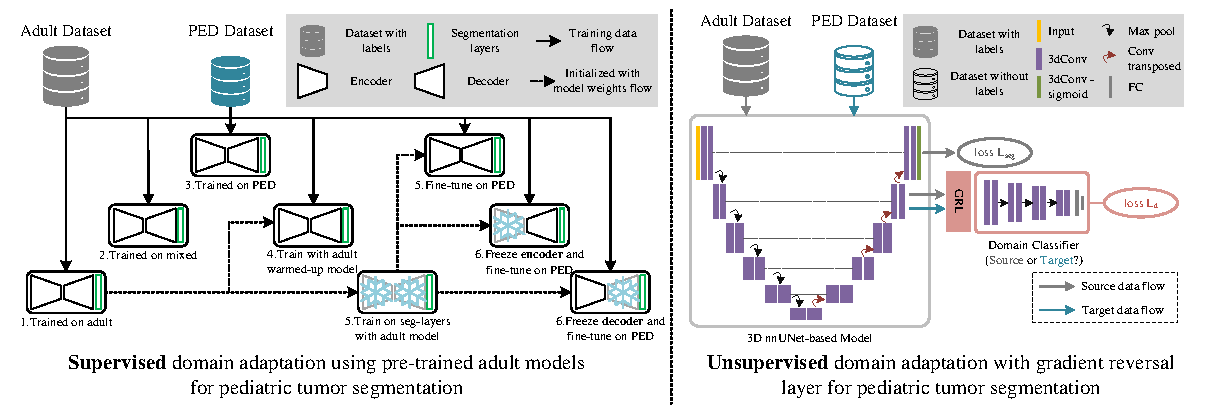
\includegraphics[width=\textwidth]{figure1.pdf}
% \caption{A figure caption is always placed below the illustration.
% Please note that short captions are centered, while long ones are
% justified by the macro package automatically.} \label{fig1}
% \end{figure}
In domain adaptation (DA), the objective is to learn a model from a source domain $\mathcal{D}_s$ and apply it to a related but different target domain $\mathcal{D}_t$ for the same task ($\mathcal{T}_s = \mathcal{T}_t$). %A domain $\mathcal{D}$ is characterized by a feature space $\mathcal{X}$ and a probability distribution $P(\mathcal{X})$ defined over $\mathcal{X}$. Meanwhile, a task $\mathcal{T}$ is defined by a label space $\mathcal{Y}$ and a prediction function $f(x) = P(y|x)$ for $x\in \mathcal{X}, y \in \mathcal{Y}$ \cite{pan2009survey,karimi2021transfer}. Depending on the availability of target labels $Y_t$, DA can be further categorized into supervised (with labeled databases $S=(X_s, Y_s)$ and $T=(X_t, Y_t)$) and unsupervised (with labeled database $S=(X_s, Y_s)$ and unlabeled database $T=(X_t)$) settings. 
In this study, we focus on UDA and use supervised domain adaptation (SDA) to establish upper-bound and baseline models.

%setting. However, we also implemented supervised domain adaptation (SDA) settings to establish baseline and upper bound models when fully annotated pediatric (PED) data being provided.

\begin{figure}[!t]
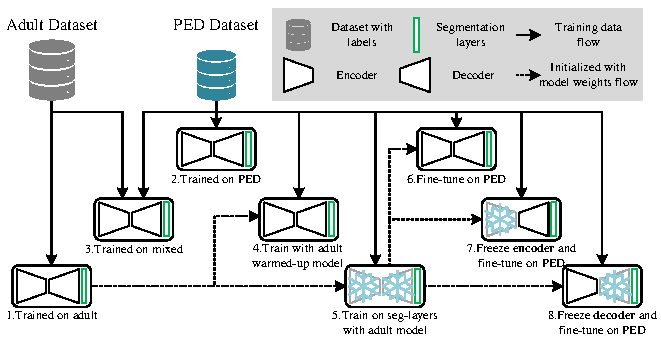
\includegraphics[width=\textwidth]{SDA.pdf}
\caption{Different strategies to obtain upper-bound and baseline models when assuming fully-annotated pediatric (PED) data are provided.} \label{fig:SDA}
\end{figure}
\subsection{Supervised Baseline Models}\label{sec:SDA}

Despite their differences, adult and pediatric tumors share relevant characteristics. Thus, using abundant annotated adult data during training should be beneficial for pediatric tumor segmentation \cite{boyd2023expert}.
In case manual annotations of pediatric images are available, a standard procedure is to apply transfer learning from adult to pediatric gliomas by combining the two datasets during training \cite{goodfellow2016deep,amod2023bridging}. This combination can be performed in different ways. 

Fig. \ref{fig:SDA} shows the 8 different supervised models. Models 1-3 in Fig. \ref{fig:SDA} train 3D nn-UNets from scratch using either or both datasets. In turn, models 5-8 use standard transfer learning strategies. First, model 5 is trained only on task-related layers, based on the pre-trained nn-UNet for adult tumor segmentation as the feature extractor. Then different parts of the network are fine-tuned with pediatric data, with lower learning rates and fewer epochs in models 6-8. Model 4 is somewhat in the middle of the two approaches, where the whole network is retrained using pediatric data after pretraining with adult data. % involving training from scratch with pediatric data but initializing weights using the pre-trained nn-UNet for adult tumor segmentation.




% Jingru's version
%When an annotated pediatric database becomes available, the most straightforward approach to improving segmentation accuracy is to retrain models on this dataset. However, as discussed earlier, adult gliomas share many visual similarities with pediatric gliomas. To capitalize on these similarities, a common approach is to pre-train a model on an adult source domain and subsequently fine-tune it on the pediatric target domain \cite{goodfellow2016deep}. 

%Due to privacy concerns often limiting access to data in medical applications, the practice of sharing pre-trained weights and transferring knowledge through them has become increasingly popular in medical fields. With this in mind, we designed our study to obtain baseline and upper-bound models based on different assumptions regarding accessibility to the source dataset. These models serve as benchmarks for comparison with UDA experiments and provide a comprehensive understanding of DA from adult to pediatric glioma segmentation in response to different scenarios in practice. Firstly, assuming access to an adult dataset, we trained three models using different dataset compositions, as illustrated in Fig. \ref{fig:SDA} (i.e., models 1-3 in Fig. \ref{fig:SDA}). Conversely, in scenarios where actual adult data is not available and only pre-trained weights are accessible, we explored five strategies to leverage knowledge from the adult domain (i.e., models 4-8 in Fig. \ref{fig:SDA}). Further implementation details are provided in the supplementary materials.

\subsection{Unsupervised Domain Adaptation for Pediatric Brain Tumor Segmentation}
\begin{figure}[!t]
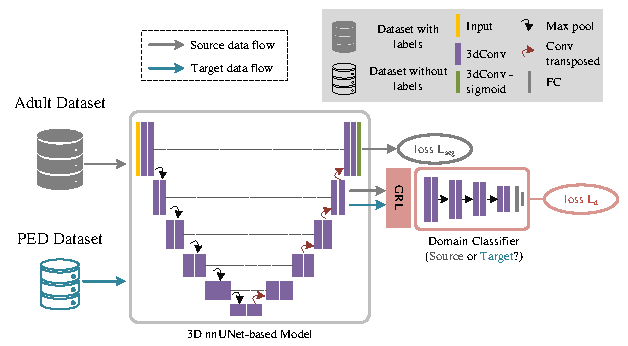
\includegraphics[width=\textwidth]{UDA.pdf}
\caption{The proposed DA-nnUNet comprises a 3D nnUNet-based backbone and a domain classifier. UDA is facilitated by integrating a gradient reversal layer (GRL) before the domain classifier. %During forward propagation, the GRL copies the input, while during backpropagation, it multiplies the gradient by a negative hyperparameter $\alpha$. This adversarial mechanism encourages the features passed to the domain classifier to become domain-invariant. Notably, the final stage of the UNet decoder is responsible for the segmentation task, minimizing segmentation loss $L_{seg}$ on source samples, while the domain classifier minimizes a domain classification loss $L_{d}$ across both domains.
} \label{fig:UDA}
\end{figure}
As illustrated in Fig. \ref{fig:UDA}, the proposed architecture consists of a 3D nnUNet-based backbone and a domain classifier. During forward propagation, the GRL \cite{ganin2016domain} acts as an identity function, while during backpropagation, it multiplies the gradient by a negative value $\alpha$. This adversarial mechanism encourages the features passed to the domain classifier to become domain-invariant. At the final stage of the UNet decoder, which is responsible for the segmentation task, the segmentation loss $L_{seg}$ is minimized only on adult samples, while the domain classifier minimizes a domain classification loss $L_{d}$ across both domains.

%The inclusion of a domain classifier stems from principles of domain adaptation, which suggest that effective domain transfer requires predictions based on features that do not distinguish between the source and target domains \cite{ben2006analysis}. This concept was initially introduced in neural architectures in \cite{ganin2016domain} for natural image classification tasks, employing a gradient reversal layer (GRL) to learn domain-invariant intermediate features for the final task. Similar efforts have been made to extend this concept to natural image segmentation \cite{bolte2019unsupervised} and 3D medical binary segmentation problems \cite{kamnitsas2017unsupervised}. We adapted this approach to the 3D region-based brain tumor segmentation problem, which, to the best of our knowledge, has not been previously explored.
 
The success of achieving domain adaptation with our model hinges on carefully balancing model learning between segmentation and domain classification tasks. Overfitting to the segmentation task may hinder domain adaptation, causing the model to excel only in source domain segmentation. Conversely, overfitting to the classification task may compel the model to prioritize learning domain-invariant features to deceive the classifier, potentially sacrificing segmentation performance. To address these concerns, we introduced several strategies to better balance the two tasks.

\textbf{Inclusion of domain classifier weight in loss}: The total loss comprises two primary components: a segmentation loss $L_{seg}$ and a domain classifier loss $L_d$. We employed a combination of pseudo-Dice loss and binary cross-entropy loss as $L_{seg}$, akin to the default loss function in nnU-Net. For $L_d$, we utilized cross-entropy loss for the one-hot with two domain labels. The total loss is represented as follows:

\begin{equation}
    L_{total} = \sum_{x\in \mathcal{D}_s} L_{seg}(\hat{y}, y) + \lambda \sum_{x\in (\mathcal{D}_s \cup \mathcal{D}_t)} L_{d}(\hat{d}, d),
\end{equation}
where $\lambda$ denotes the domain classifier weight, controlling the relative importance of the segmentation and classification tasks; $\hat{d}$ and $d$ are the predicted and actual domain labels; and $\hat{y}$ and $y$ represent the predicted and ground truth segmentation masks for the adult dataset $\mathcal{D}_s$, respectively. We assume no annotations are available for the pediatric dataset $\mathcal{D}_t$, so they are not considered in $L_{seg}$. 

\textbf{Dynamic scheduler for $\alpha$ in GRL}: A crucial component is the adjustment of $\alpha$ in the GRL, which dictates the strength of feature adaptation in response to the domain classifier. Following \cite{kamnitsas2017unsupervised}, we implemented a truncated ramp function in which the value of $\alpha$ grows linearly from 0 at epoch $e_{min}$ to $\alpha_{max}$ at epoch $e_{max}$. $e_{min}$ is selected such that the accuracy of the classifier is very high. Ideally, such an accuracy should decay to a chance level at $e_{max}$. Finally, we maintain $\alpha$ at its maximum value $\alpha_{max}$ to focus on refining further the segmentation. 



%three-stage scheduler to dynamically modulate the value of $\alpha$ based on the maximum epoch number $ep_{max}$. Initially, we allow the segmentation backbone and domain classifier to independently learn their respective tasks until $p1$*$ep_{max}$ epochs by setting $\alpha=0$. Subsequently, as both components become more proficient in their tasks, we progressively reduce $\alpha$ until $p2$*$ep_{max}$ epochs to enable domain adaptation. For this, $\alpha$ is adjusted according to $\alpha=\alpha_{max}\frac{p_{curr}-p1}{p2-p1}$, where $p_{curr}=\frac{ep_{curr}}{ep_{max}}$, $ep_{curr}$ is current epoch. Finally, when the learned features effectively deceive the domain classifier, we maintain $\alpha$ at its maximum value $\alpha_{max}$ to focus on refining the segmentation. 

% \textbf{Scalable domain classifier architecture}: 

\section{Experimental Setting}
\subsection{Datasets}
% \begin{table}[t]
% \caption{Datasets used in the experiments. Each subset was randomly sampled from the raw datasets.}\label{tab:dataset}
% \begin{tabular}{ccccc}
% \hline
% \textbf{Dataset} &
%   \textbf{Data Subset} &
%   \textbf{\# Subjects} &
%   \textbf{\begin{tabular}[c]{@{}c@{}}Labels Used\\ (Supervised)\end{tabular}} &
%   \textbf{\begin{tabular}[c]{@{}c@{}}Labels Used\\ (Unsupervised)\end{tabular}} \\ \hline
% \multirow{2}{*}{BraTS Adult Glioma} & $\mathcal{D}_{\text{Adult}}^{\text{train}}$ & 1000 & \Checkmark & \Checkmark \\
%                                     & $\mathcal{D}_{\text{Adult}}^{\text{test}}$ & 251  & \Checkmark & \Checkmark \\
% \multirow{2}{*}{BraTS-PEDs}         & $\mathcal{D}_{\text{PED}}^{\text{train}}$ & 79   & \Checkmark &  \\
%                                     & $\mathcal{D}_{\text{PED}}^{\text{test}}$ & 20   & \Checkmark & \Checkmark \\ \hline
% \end{tabular}
% \end{table}

\begin{table}[t]
\caption{Datasets used in the experiments.}\label{tab:dataset}
\begin{tabular}{ccccc}
\hline
\textbf{Dataset} & \textbf{Data Subset} & \textbf{\# Subjects} & \textbf{\begin{tabular}[c]{@{}c@{}}Labels Used\\ (Supervised)\end{tabular}} & \textbf{\begin{tabular}[c]{@{}c@{}}Labels Used\\ (Unsupervised)\end{tabular}} \\ \hline
BraTS Adult Glioma & $\mathcal{D}_{\text{Adult}}^{\text{source}}$ & 1251 & \Checkmark & \Checkmark \\
BraTS-PEDs         & $\mathcal{D}_{\text{PED}}^{\text{target}}$ & 99   & \Checkmark &  \\
\hline
\end{tabular}
\end{table}

\begin{figure}[t]
     \centering
     %\begin{subfigure}[b]%{0.48\textwidth}
         \centering
         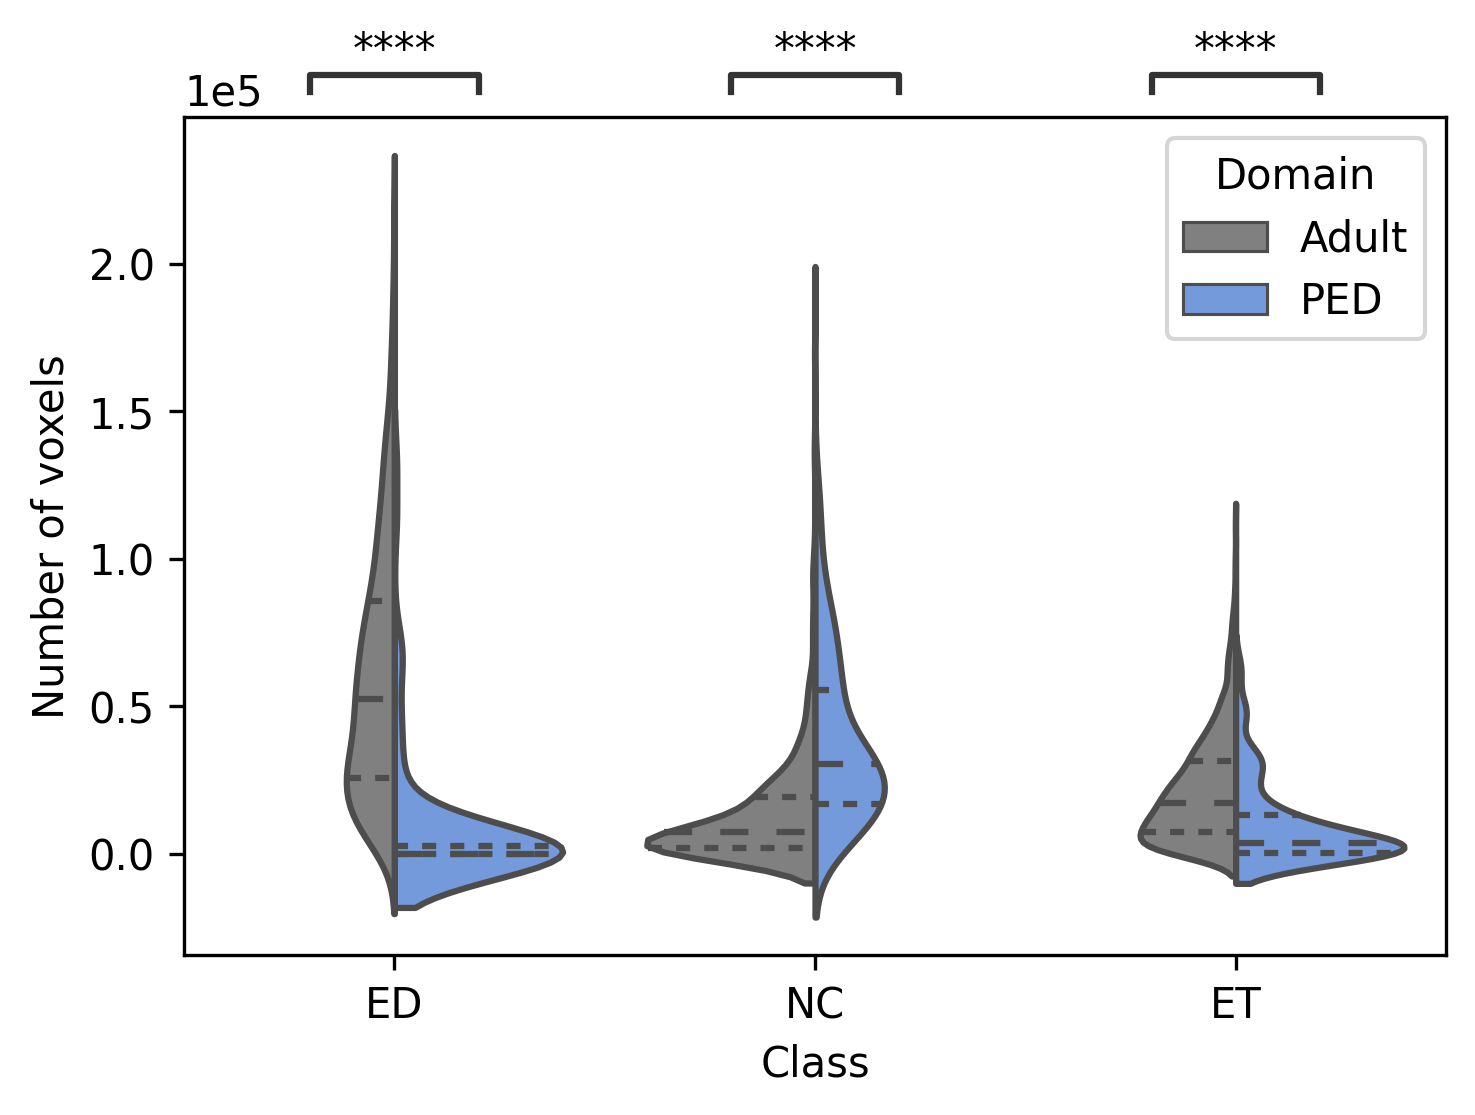
\includegraphics[width=0.48\textwidth]{Volumes1.png}
     %\end{subfigure}
     \hfill
     %\begin{subfigure}[b]{0.48\textwidth}
         \centering
         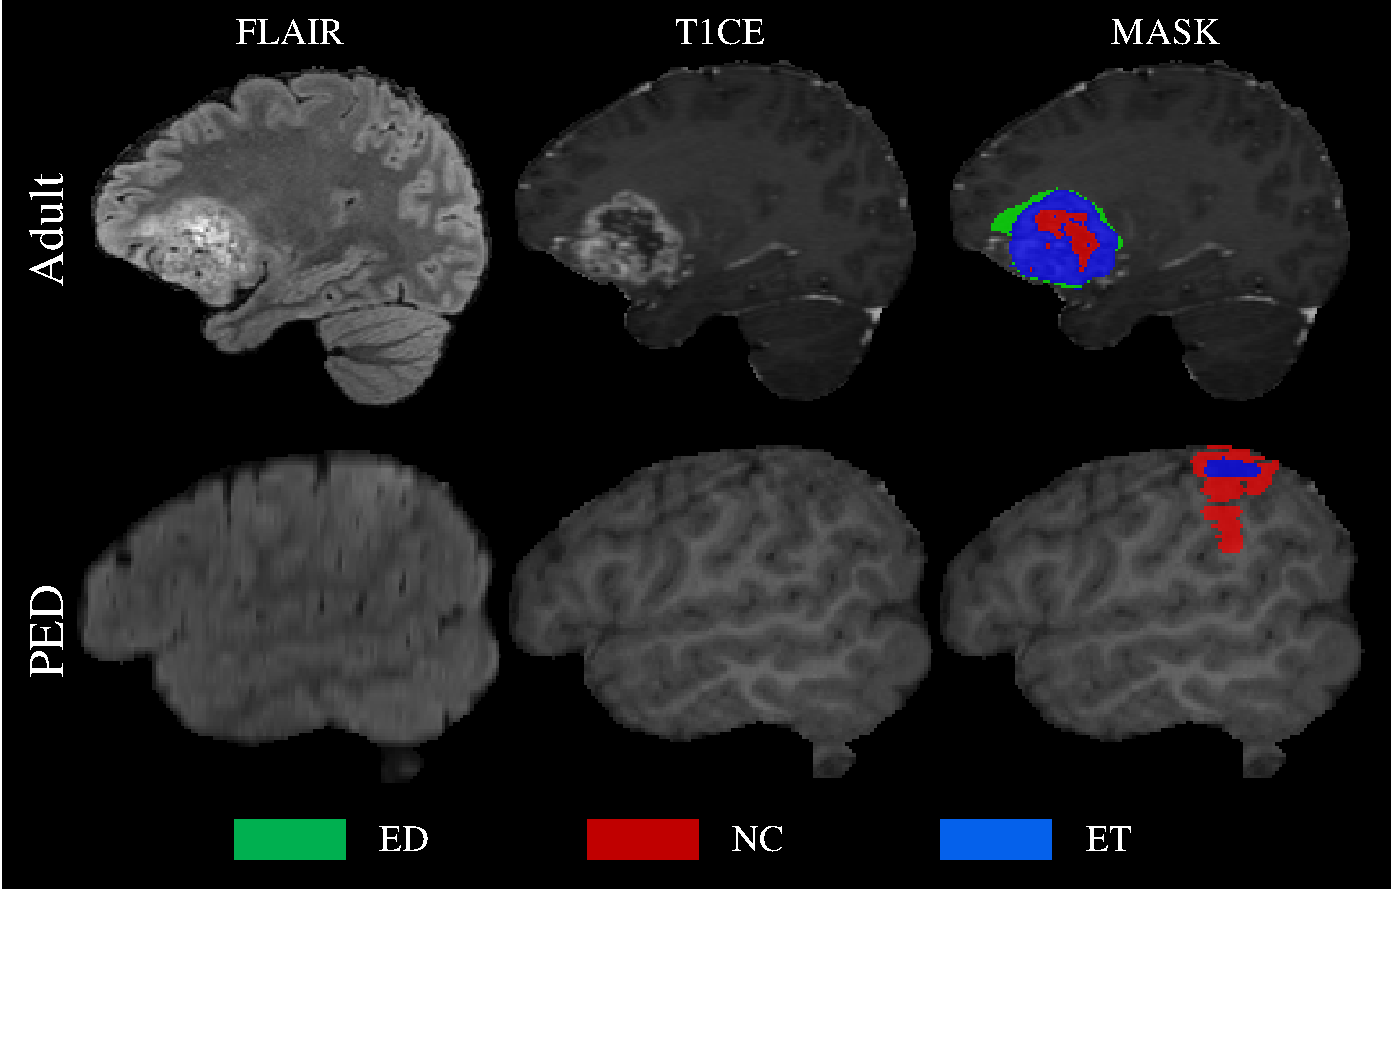
\includegraphics[width=0.48\textwidth]{examples2.pdf}
     %\end{subfigure}
\caption{Distribution of tumor sizes (left) and examples of the appearance of adult and pediatric tumors on FLAIR and T1w after contrast (T1CE) (right).
%intensities between BraTS adult glioma and BraTS-PEDs datasets.
} \label{fig:domaindiff}
\end{figure}

We utilized two databases provided by the BraTS challenge organizers: the BraTS 2021 adult glioma dataset \cite{menze2014multimodal}, and the BraTS-PEDs 2023 dataset \cite{kazerooni2023brain}. All data underwent identical preprocessing steps, including conversion to NifTI format, skull stripping, defacing, co-registration to the SRI24 anatomical template, and resampling to isotropic resolution. Subsequently, the data were cropped to a size of [240, 240, 155]. Each dataset included four mpMRIs: pre- and post-gadolinium T1-weighted (T1w), T2-weighted (T2w), and T2 fluid attenuated inversion recovery (FLAIR) images. Additionally, expert annotated segmentation masks were provided, delineating three classes: enhancing tumor (ET), non-enhancing component (NC), and edema (ED).

We employed the training datasets to validate our method for the segmentation of three subregions: whole tumor (WT: ET+NC+ED), tumor core (TC: ET+NC), and enhancing tumor (ET). Details regarding each domain are summarized in Table \ref{tab:dataset}. All models using PED data were trained using 5-fold cross validation (CV), while \textit{adult} model was trained using all adult data. %For establishing baselines and upper bounds, we utilized the supervised settings described in Sect. \ref{sec:SDA}. In the UDA, only labels from the source domain were utilized, as indicated in the last column of Table \ref{tab:dataset}. 
As shown in Fig. \ref{fig:domaindiff}, there are significant disparities (i.e., \textit{domain shift}) between adult and pediatric gliomas for tumor subregion sizes and appearance. Note that in the BraTS-PEDs set, 11 out of 99 cases lack the ET region (compared to 33 out of 1251 cases in the BraTS adult glioma set), while 42 out of 99 cases lack the ED region (compared to only 1 out of 1251 cases in the BraTS adult glioma set). 

\subsection{Implementation}
Benefiting from the auto-configuring capability of nnU-Net, many preprocessing, postprocessing, and architecture hyperparameters can be robustly handled by nnU-Net's default strategies. However, to harness the DA capability of our proposed model, the introduction of a domain classifier necessitates careful selection of additional hyperparameters, along with extra effort to tailor current default segmentation configuration strategies for UDA. 

Firstly, the architecture of the domain classifier must be designed and adjusted to accommodate the complexity of nnU-Net. We introduced the same block structure (i.e., double convolutional layers followed by max pooling) as in the backbone of nnU-Net. Two hyperparameters can be freely adjusted to modify the depth of the domain classifier: i) the number of blocks (set to 4 in our experiments); ii) the number of channels for convolutional layers and the final fully-connected (FC) layer (set to 100).
Secondly, as discussed previously, the scheduler for $\alpha$ in the GRL involves three hyperparameters: $e_{min} = 100$, $e_{max} = 350$, and $\alpha_{max}=3$. Additionally, we observed that the default deep supervision (DS) strategy in nnU-Net tends to prioritize the segmentation task, potentially bypassing the learning of domain-invariant features and leading to an imbalance between segmentation and classification tasks. Therefore, we disabled DS in our proposed model training.
The hyperparameter $\lambda$ is set to 0.01, the batch size is set to 4, the maximum number of epochs is set to 500, and a domain-balanced dataloader is utilized to prevent failure in domain classification. Finally, the learning rate is implemented following the same approach as described in \cite{ganin2016domain}, with an initial value of 0.01.%However, it is important to note that optimal settings are not yet fully explored and may vary depending on the specific application.

% JR: June/20 I update results to 5 CV
\begin{table}[t]
\caption{Comparison of methods using 5-fold cross-validation (5CV) (excluding models 1 and 1$^*$).
The models are ranked separately based on whether they have access to adult source data for training, or if deep supervision (DS) was deactivated (marked with $^*$). The best in each category is highlighted in bold.}\label{tab:SDA}
\centering
\begin{tabular}{cccc|ccc|ccc|ccc}
\hline
\multirow{2}{*}{\textbf{Model}} & \multicolumn{3}{c|}{\textbf{mean DSC}}           & \multicolumn{3}{c|}{\textbf{mean HD95}}         & \multicolumn{3}{c|}{\textbf{median DSC}}         & \multicolumn{3}{c}{\textbf{median HD95}}        \\ \cline{2-13} 
                                & ET             & TC             & WT             & ET              & TC            & WT            & ET             & TC             & WT             & ET             & TC            & WT            \\ \hline
1                               &  \textbf{0.583}& 0.522& 0.900&  \textbf{58.77}& 36.11& 4.82&  \textbf{0.742}& 0.549& 0.913&  \textbf{4.12}& 13.49& 3.00\\
2                               & 0.547&  \textbf{0.872}& 0.897& 62.70&  \textbf{5.53}& 4.83& 0.708& 0.915& 0.924& 6.40&  \textbf{3.61}& 3.16\\
3                               & 0.575& 0.854&  \textbf{0.908}& 66.18& 9.38&  \textbf{4.22}& 0.716&  \textbf{0.918}&  \textbf{0.927}& 4.36&  \textbf{3.61}&  \textbf{2.83}\\ \hline
4                               & 0.579& 0.874& 0.898& 66.30& 8.78& 4.55& 0.713&  \textbf{0.914}&  \textbf{0.922}& 5.39&  \textbf{3.32}&  \textbf{3.00}\\
5                               & 0.577& 0.852& 0.902& 52.66& 6.42& 4.66&  \textbf{0.732}& 0.895& 0.917& 5.00& 4.47&  \textbf{3.00}\\
6                               &  \textbf{0.584}&  \textbf{0.879}&  \textbf{0.906}&  \textbf{51.79}&  \textbf{5.23}&  \textbf{4.26}& 0.712& 0.910&  \textbf{0.922}&  \textbf{4.24}& 3.61&  \textbf{3.00}\\
7                               & 0.582& 0.869& 0.901& 55.25& 5.54& 4.31& 0.702& 0.906& 0.920& 4.47& 3.74&  \textbf{3.00}\\
8                               & 0.574& 0.875& 0.903& 62.23& 5.65& 4.54& 0.718& 0.908& 0.921& 5.00& 3.74&  \textbf{3.00}\\ \hline
1$^*$                      & 0.571& 0.526& 0.890& 59.61& 22.25& 7.07&  \textbf{0.739}& 0.555& 0.909&  \textbf{4.47}& 13.49& 3.61\\
2$^*$                       & 0.511& 0.855& 0.886& 50.62& 6.24& 5.37& 0.631&  \textbf{0.909}&  \textbf{0.921}& 7.55&  \textbf{3.74}& 3.16\\
3$^*$                       &  \textbf{0.575}&  \textbf{0.861}&  \textbf{0.909}&  \textbf{45.50}&  \textbf{5.47}&  \textbf{5.16}& 0.721& 0.905& 0.920& 5.10&  \textbf{3.74}&  \textbf{2.83}\\ \hline
\textbf{UDA}             & 0.580& 0.846& 0.892& 50.87& 16.55& 8.90& 0.713& 0.916& 0.923& 4.24& 3.32& 3.00\\ \hline
\end{tabular}
\end{table}

\section{Results and Discussion}
We evaluated the performance of models on $\mathcal{D}_{\text{PED}}^{\text{target}}$ using average and median DSCs along with the 95th percentile Hausdorff distance (HD95).
%\footnote{We used the script provided by the BraTS 2023 challenge for performing all metric calculations. \url{https://github.com/rachitsaluja/BraTS-2023-Metrics}}. 
The results of all models are summarized in Table \ref{tab:SDA}. %Additionally, we conducted statistical tests using pairwise t-tests to compare three baseline models without DS (models 1$^*$-3$^*$) with the proposed DA-nnUNet model, as illustrated in Fig.~\ref{fig:results}. %, while the results of UDA are presented in Table \ref{tab:UDA}.
%Additionally, to provide statistical robustness to the conclusions inferred from the results, we performed pairwise t-tests over the segmentation metrics collected in different experiments.

% \begin{table}[t]
% \caption{Comparison of methods on $\mathcal{D}_{\text{PED}}^{\text{test}}$.
% %Comparison of baseline and upper-bound models on $\mathcal{D}_{\text{PED}}^{\text{test}}$ described in Fig. \ref{fig:SDA}. 
% The models are ranked separately based on whether they have access to adult source data for training, or if deep supervision was deactivated (marked with *). The best in each category is highlighted in bold.}\label{tab:SDA}
% \centering
% \begin{tabular}{cccc|ccc|ccc|ccc}
% \hline
% \multirow{2}{*}{\textbf{Model}} & \multicolumn{3}{c|}{\textbf{mean DSC}}           & \multicolumn{3}{c|}{\textbf{mean HD95}}         & \multicolumn{3}{c|}{\textbf{median DSC}}         & \multicolumn{3}{c}{\textbf{median HD95}}        \\ \cline{2-13} 
%                                 & ET             & TC             & WT             & ET              & TC            & WT            & ET             & TC             & WT             & ET             & TC            & WT            \\ \hline
% 1                               & \textbf{0.470} & 0.562          & 0.906          & \textbf{100.34} & 15.18         & 4.13          & \textbf{0.615} & 0.650          & 0.921          & \textbf{9.52}  & 11.06         & 2.91          \\
% 2                               & 0.379          & 0.896          & 0.902          & 123.54          & 4.33          & 4.07          & 0.279          & 0.926          & \textbf{0.939} & 17.34          & 3.00          & 2.83          \\
% 3                               & 0.430          & \textbf{0.899} & \textbf{0.917} & 105.44          & \textbf{3.85} & \textbf{3.08} & 0.460          & \textbf{0.940} & 0.917          & 14.04          & 3.00          & \textbf{2.45} \\ \hline
% 4                               & 0.389          & \textbf{0.907} & 0.912          & 107.79          & \textbf{3.80} & \textbf{3.42} & 0.333          & \textbf{0.931} & \textbf{0.941} & 11.00          & \textbf{2.91} & 2.83          \\
% 5                               & 0.413          & 0.861          & 0.909          & \textbf{71.69}  & 5.93          & 3.97          & 0.441          & 0.902          & 0.925          & 11.82          & 3.16          & 2.83          \\
% 6                               & 0.423          & 0.892          & 0.904          & 87.63           & 4.53          & 4.05          & 0.478          & 0.923          & 0.930          & 15.07          & 3.00          & 2.91          \\
% 7                               & 0.411          & 0.900          & \textbf{0.918} & 88.17           & 4.13          & 3.45          & 0.497          & 0.910          & 0.925          & 16.12          & 3.00          & \textbf{2.64} \\
% 8                               & \textbf{0.451} & 0.877          & 0.895          & 103.31          & 5.46          & 4.54          & \textbf{0.648} & 0.913          & 0.935          & \textbf{10.41} & 3.08          & \textbf{2.64} \\ \hline
% 1$^*$                      & \textbf{0.477} & 0.544          & 0.893          & 85.10           & 15.01         & 4.75          & \textbf{0.598} & 0.555          & 0.926          & \textbf{10.28} & 13.43         & 2.88          \\
% 2$^*$                       & 0.366          & 0.875          & 0.894          & 73.95           & 5.03          & 4.09          & 0.257          & 0.915          & \textbf{0.936} & 16.68          & \textbf{2.91} & 2.83          \\
% 3$^*$                       & 0.435          & \textbf{0.908} & \textbf{0.925} & \textbf{54.17}  & \textbf{3.62} & \textbf{3.21} & 0.486          & \textbf{0.927} & 0.934          & 11.38          & 3.24          & \textbf{2.34} \\ \hline
% \textbf{Ours}             & 0.409          & 0.889          & 0.903          & 100.93          & 4.12          & 3.76          & 0.364          & 0.930          & 0.938          & 12.12          & 2.91          & 2.45          \\ \hline
% \end{tabular}
% \end{table}

% From the results of Table \ref{tab:SDA}, %both the mean and median metrics were reported, acknowledging that the mean can be disproportionately influenced by outliers, while the median provides a more representative measure of the model's performance across typical cases. 
The results revealed that model 1, trained solely on adult data, mainly faces challenges in accurately segmenting the TC region, as evidenced by a decrease in mean DSC from 0.872 to 0.522 compared to model 2. In comparison to model 2, which was trained on a limited dataset of pediatric cases, model 3 benefits from combining both pediatric and adult datasets, resulting in improved median DSC and HD95 metrics due to its exposure to diverse domain characteristics. Since we deactivated the DS in the proposed UDA method, we also trained models 1-3 without DS (models 1$^*$-3$^*$) for fair comparison. As shown, these models perform very similarly to models 1 and 3 with DS with enough training data. Notably, models 3 and 3$^*$ are regarded as practical upper bounds for any DA model. Supervised DA models 4-8 achieve comparable results to the upper bound model trained with both datasets. Lastly, the proposed UDA method obtains segmentation accuracies which are close to the upper bound model 3$^*$ without requiring any annotations from pediatric domain. This underscores the necessity and efficacy of the adaptation.

% Regarding TC and WT, training the nnU-Net model with a combined dataset comprising adult glioma and pediatric brain tumors (model 3 and 3$^*$) resulted in a superior segmentation performance on pediatric cases. % in the WT and TC regions, while the model trained only on adult cases performed slightly better in the ET region. 
% This observation can be explained by the model's exposure to diverse domain characteristics during the training phase, combining domain-specific feature extraction from pediatric cases and leveraging shared domain features.
% %The lower part of Table \ref{tab:SDA} presents the segmentation results for different experimental setups, all derived from an initial model pre-training on adult subjects as described in Sect. \ref{sec:SDA}. %: Model 4 and 5 adopt a transfer learning approach, while Model 6,7, and 8 are derived from fine-tuning different layers of the the pre-trained nnU-Net architecture.
% Models 4-8 yield similar results, with models 4 and 7 being slightly superior to model 3. Since we deactivated the DS in the proposed method, we also trained models 1-3 without DS (models 1$^*$-3$^*$). As shown, these models perform very similarly to models 1-3 with DS. %Thus, models 1 and 3 (no DS) can be thought of as lower and upper bounds for our method. 
% We also observe that our proposed UDA method is competitive with all tested supervised baselines, particularly when compared to two adult models (models 1 and 1$^*$) in the tumor core (TC) region, where our method exhibits significant improvement (mean DSC increased by at least 0.327). This underscores the necessity and efficacy of the adaptation.
% %For this reason, models 1-3 without DS are used as baselines.


% \begin{table}[t]
% \caption{Comparison of our method's performance on $\mathcal{D}_{\text{PED}}^{\text{test}}$ with several baselines. Our proposed UDA model bridges the gap between the lower bound, where the model is trained solely on adult source domain data, and the upper bound, where the model is solely trained with data from the pediatric target domain. The best values are shown in bold, while the second-best values are underlined.}\label{tab:UDA}
% \centering
% \begin{tabular}{cccccc|cccc}
% \hline
% \multirow{2}{*}{\textbf{Model}} & \multirow{2}{*}{\textbf{Trained on}} & \multicolumn{4}{c|}{\textbf{mean DSC}} & \multicolumn{4}{c}{\textbf{mean HD95}} \\ \cline{3-10} 
%             &  & avg. & ET & TC & WT & avg. & ET & TC & WT \\ \hline
% Adult\_noDS & $\mathcal{D}_{\text{Adult}}^{\text{train}}$ &      0.6380&    0.4768&    0.5444&    0.8928&      34.95&    85.10&    15.01&    4.75\\
% PED\_noDS   & $\mathcal{D}_{\text{PED}}^{\text{train}}$ &      0.7114&    0.3659&    0.8749&    0.8935&      27.69&    73.95&    5.03&    4.09\\
% Mixed\_noDS & $\mathcal{D}_{\text{Adult}}^{\text{train}} \cup \mathcal{D}_{\text{PED}}^{\text{train}}$ &      \textbf{0.7559}&    0.4351&    0.9076&    0.9250&      20.33&    54.17&    3.62&    3.21\\
% UDA (ours)  & $\mathcal{D}_{\text{Adult}}^{\text{train}} \cup \mathcal{D}_{\text{PED}}^{\text{train}}$ &      0.7339&    0.4091&    0.8894&    0.9032&      36.27&    100.93&    4.12&    3.76\\ \hline
% \end{tabular}
% \end{table}

% \begin{table}[t]
% \caption{Comparison methods after removing cases with no or small ET region %(<200 voxels), and an outlier \textit{BraTS-PED-00008-000}. %Our proposed UDA model bridges the gap between the lower bound, where the model is trained solely on adult source domain data, and the upper bound, where the model is also trained with data from the pediatric target domain. 
% The best values are shown in bold, while the second-best values are underlined.}\label{tab:UDA}
% \centering
% \begin{tabular}{cccccc|cccc}
% \hline
% \multirow{2}{*}{\textbf{Model}} & \multirow{2}{*}{\textbf{Trained on}} & \multicolumn{4}{c|}{\textbf{mean DSC ($\uparrow$)}} & \multicolumn{4}{c}{\textbf{mean HD95 ($\downarrow$)}} \\ \cline{3-10} 
%             &  & avg. & ET & TC & WT & avg. & ET & TC & WT \\ \hline
% 1 (no DS) & $\mathcal{D}_{\text{Adult}}^{\text{train}}$ &      0.652& \underline{0.569}&    0.508&    0.881&      26.65&    57.14&    17.18&    5.64\\
% 2 (no DS)   & $\mathcal{D}_{\text{PED}}^{\text{train}}$ &      0.741&    0.488&    0.856&    0.880&      15.33&    35.31&    5.96&    4.73\\
% 3 (no DS) & $\mathcal{D}_{\text{Adult}}^{\text{train}} \cup \mathcal{D}_{\text{PED}}^{\text{train}}$ &      \textbf{0.800}&    \textbf{0.580}&    \textbf{0.900}&    \textbf{0.920}&      \textbf{5.70}&    \textbf{9.40}&    \textbf{4.02}&    \textbf{3.68}\\
% \textbf{UDA (ours)}  & $\mathcal{D}_{\text{Adult}}^{\text{train}} \cup \mathcal{D}_{\text{PED}}^{\text{train}}$ &      \underline{0.771}&    0.545&    \underline{0.875}&    \underline{0.892}&      \underline{6.36}&    \underline{9.90}&    \underline{4.79}&    \underline{4.40}\\ \hline
% \end{tabular}
% \end{table}

% \begin{figure}[t]
%      \centering
%      %\begin{subfigure}[b]{0.48\textwidth}
%          \centering
%          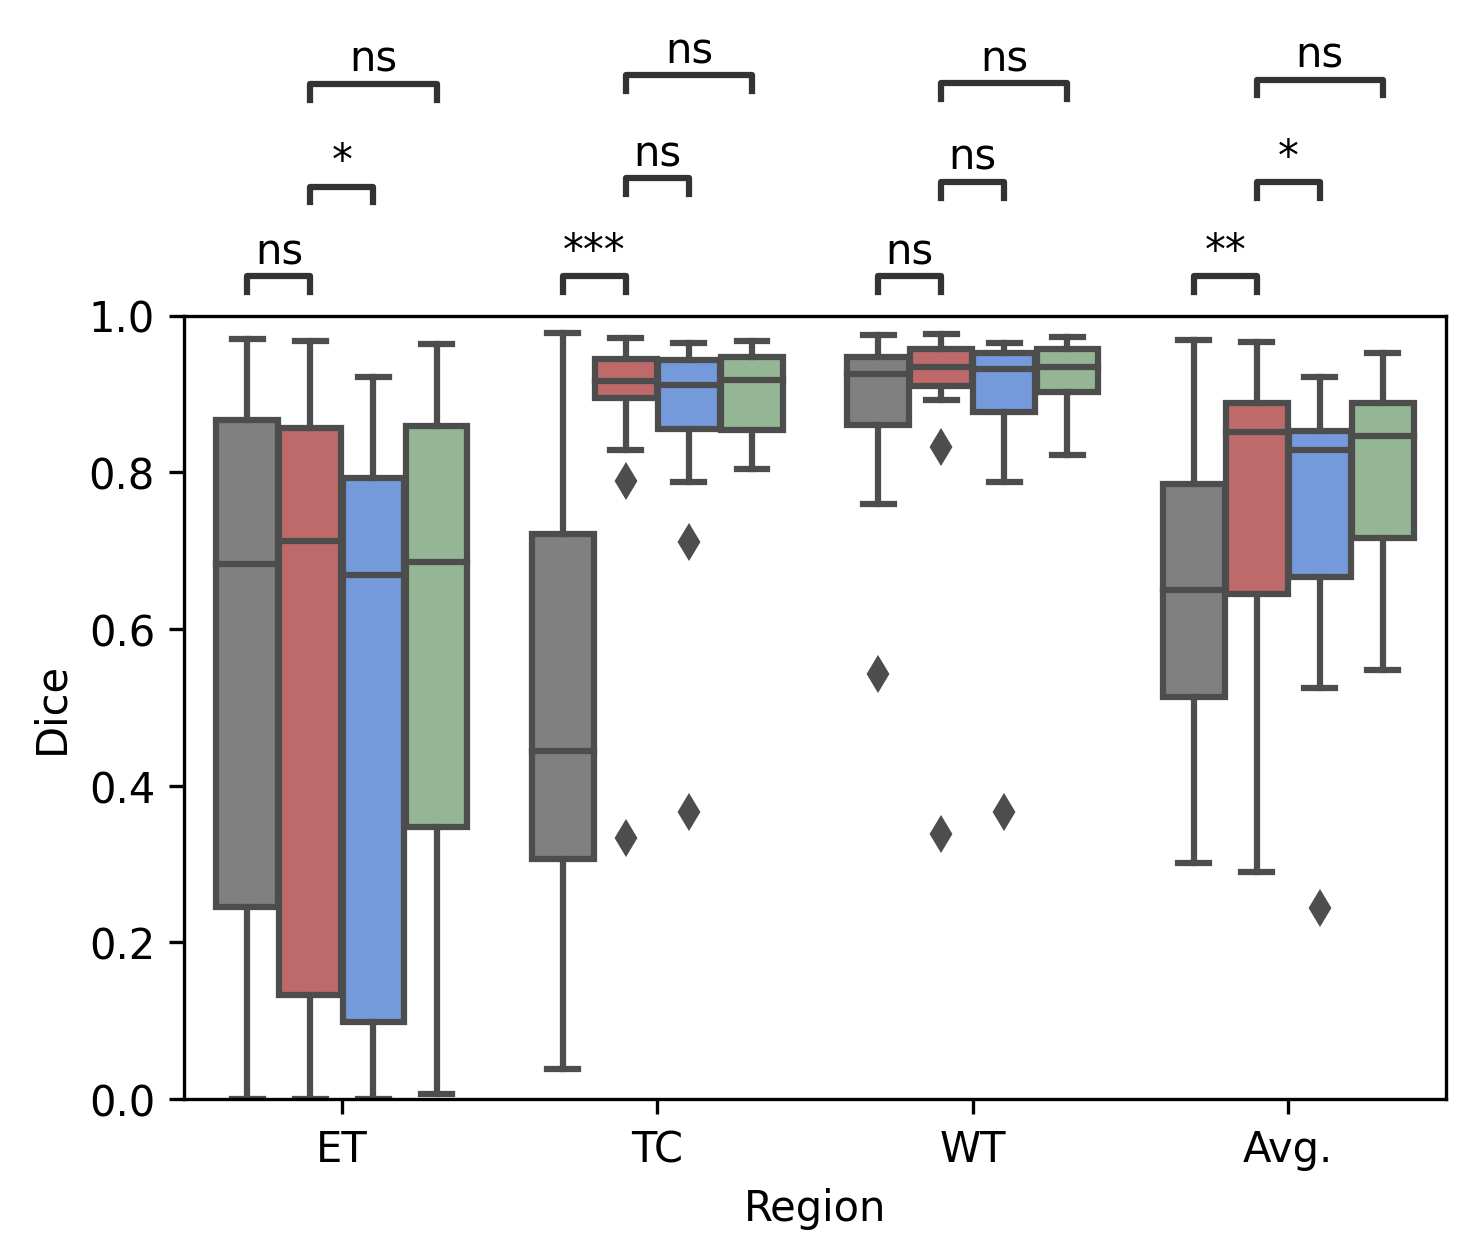
\includegraphics[width=0.48\textwidth]{Results_Unsupervised_Dice_removed.png}
%          %\caption{Tumor volume comparison}
%          \label{fig:results_GRL}
%      %\end{subfigure}
%      \hfill
%      %\begin{subfigure}[b]{0.48\textwidth}
%          \centering
%          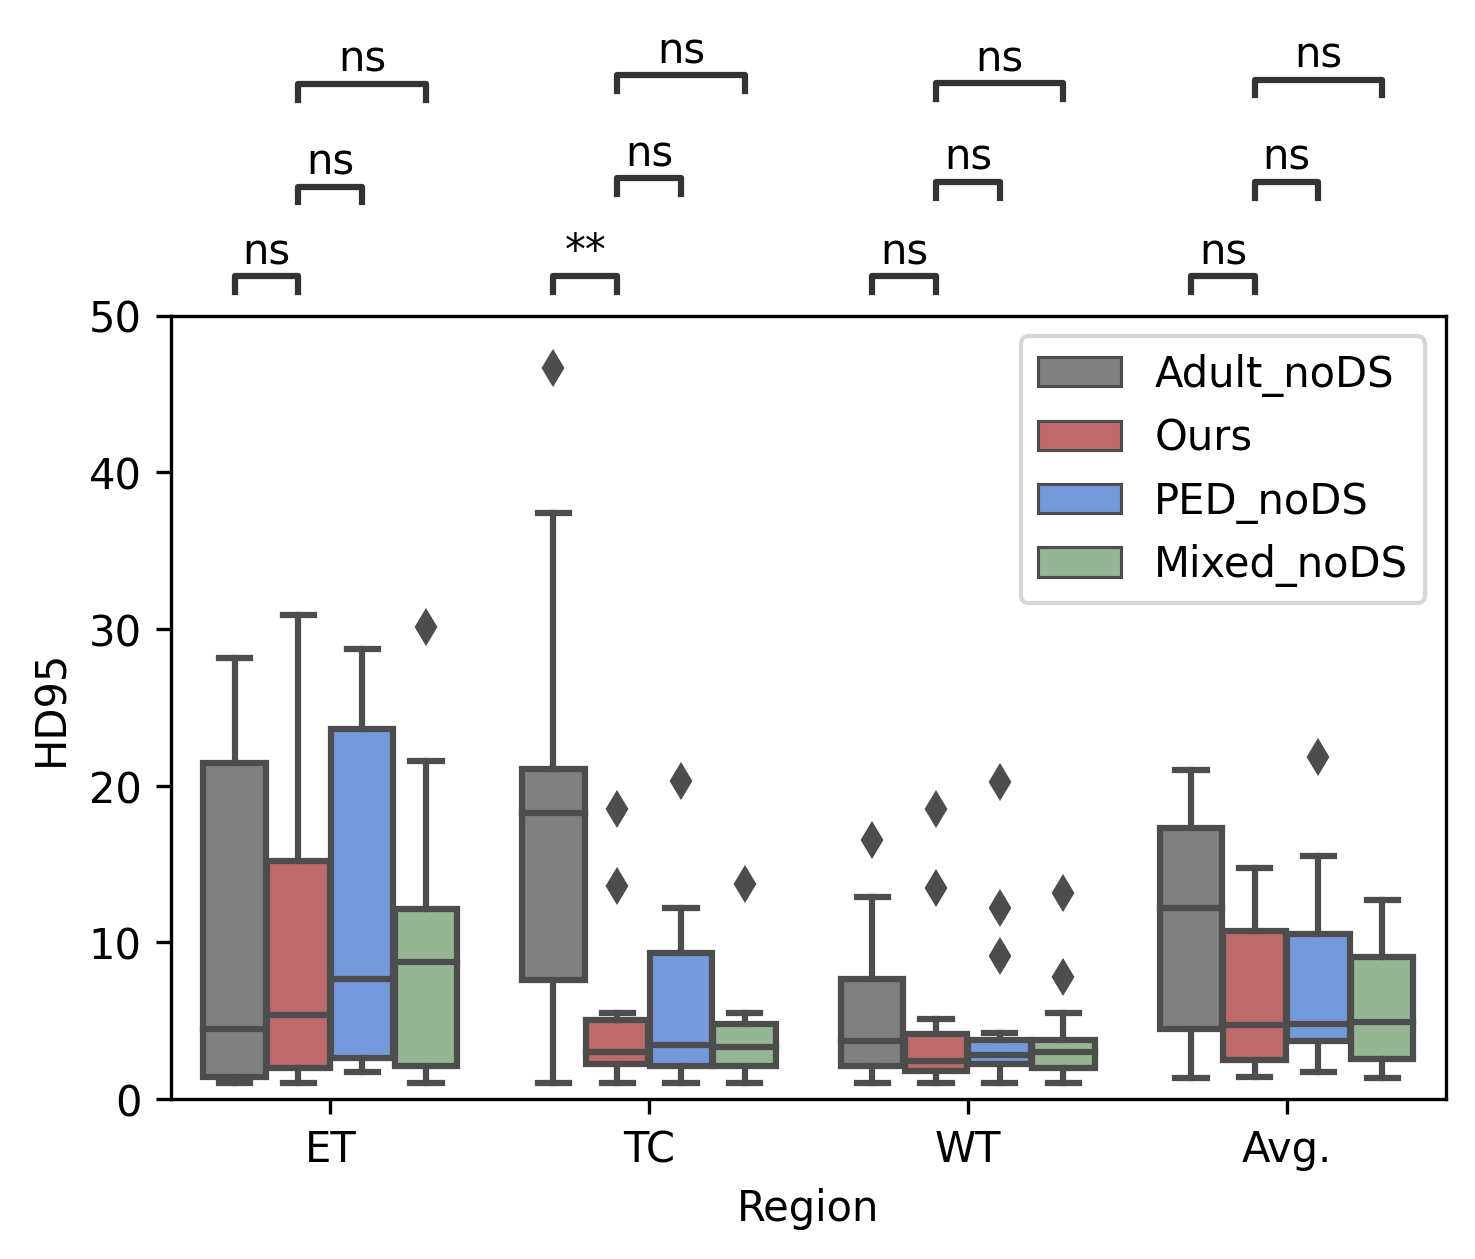
\includegraphics[width=0.48\textwidth]{Results_Unsupervised_HD95_removed_legend.png}
%          %\caption{Tumor intensity comparsion}
%          \label{fig:visual_illustration}
%      %\end{subfigure}
% \caption{Distributions of Dice scores (left) and Hausdorff distance 95 (HD95) (right) for baseline models and the proposed one.} \label{fig:results}
% \end{figure}

% \begin{table}[t]
% \caption{Comparison methods after removing cases with no or small ET region. %(<200 voxels), and an outlier \textit{BraTS-PED-00008-000}. %Our proposed UDA model bridges the gap between the lower bound, where the model is trained solely on adult source domain data, and the upper bound, where the model is also trained with data from the pediatric target domain. 
% The best values are shown in bold, while the second-best values are underlined.}\label{tab:UDA_remove}
% \centering
% \begin{tabular}{ccccc|ccc}
% \hline
% \multirow{2}{*}{\textbf{Model}} & \multirow{2}{*}{\textbf{Trained on}} & \multicolumn{3}{c|}{\textbf{mean DSC ($\uparrow$)}} & \multicolumn{3}{c}{\textbf{mean HD95 ($\downarrow$)}} \\ \cline{3-8} 
%             & & ET & TC & WT & ET & TC & WT \\ \hline
% 1$^*$ & $\mathcal{D}_{\text{Adult}}^{\text{train}}$ &  \underline{0.533}&    0.522&    0.881&  54.64&    16.51&    5.44\\
% 2$^*$  & $\mathcal{D}_{\text{PED}}^{\text{train}}$ &  0.457&    0.858&    0.881&  34.43&    5.77&    4.61\\
% 3$^*$ & $\mathcal{D}_{\text{Adult}}^{\text{train}} \cup \mathcal{D}_{\text{PED}}^{\text{train}}$ &       \textbf{0.543}&    \textbf{0.898}&    \textbf{0.919}&     \textbf{10.27}&    \textbf{4.02}&    \textbf{3.60}\\
% \textbf{UDA (ours)}  & $\mathcal{D}_{\text{Adult}}^{\text{train}} \cup \mathcal{D}_{\text{PED}}^{\text{train}}$ &      0.511&    \underline{0.875}&    \underline{0.892}&      \underline{32.66}&    \underline{4.73}&    \underline{4.28}\\ \hline
% \end{tabular}
% \end{table}

\begin{table}[t]
\caption{Comparison methods after removing cases with no or small ET region. %(<200 voxels), and an outlier \textit{BraTS-PED-00008-000}. %Our proposed UDA model bridges the gap between the lower bound, where the model is trained solely on adult source domain data, and the upper bound, where the model is also trained with data from the pediatric target domain. 
The best values are shown in bold, while the second-best values are underlined.}\label{tab:UDA_remove}
\centering
\begin{tabular}{cccc|ccc|ccc|ccc}
\hline
\multirow{2}{*}{\textbf{Model}} & \multicolumn{3}{c|}{\textbf{mean DSC}}           & \multicolumn{3}{c|}{\textbf{mean HD95}}         & \multicolumn{3}{c|}{\textbf{median DSC}}         & \multicolumn{3}{c}{\textbf{median HD95}}        \\ \cline{2-13} 
                                & ET             & TC             & WT             & ET              & TC            & WT            & ET             & TC             & WT             & ET             & TC            & WT            \\ \hline
1$^*$                      & \underline{0.661}& 0.543& 0.894& 27.50& 14.75& 7.29&  \textbf{0.768}& 0.522& 0.908&  \underline{3.61}& 13.49& 3.74\\
2$^*$                       & 0.616& 0.857& 0.894& 14.05& 6.36& 5.27& 0.729&  0.900&  0.916& 5.10&  4.24& 3.46\\
3$^*$                       &  \textbf{0.685}& \underline{0.863}&  \textbf{0.913}&  \textbf{12.98}&  \textbf{5.74}&  5.46& \underline{0.760}& \underline{0.902}& \underline{0.918}& \underline{3.61}&  \underline{4.12}&  \textbf{3.00}\\ 
\textbf{UDA}             & 0.660& \textbf{0.864}& \underline{0.908}& \underline{13.22}& \underline{5.90}& \textbf{5.15}& 0.757& \textbf{0.913}& \textbf{0.919}& \textbf{3.16}& \textbf{3.74}& \underline{3.16}\\ \hline
\end{tabular}
\end{table}

\begin{figure}[!h]
     \centering
     %\begin{subfigure}[b]{0.48\textwidth}
         \centering
         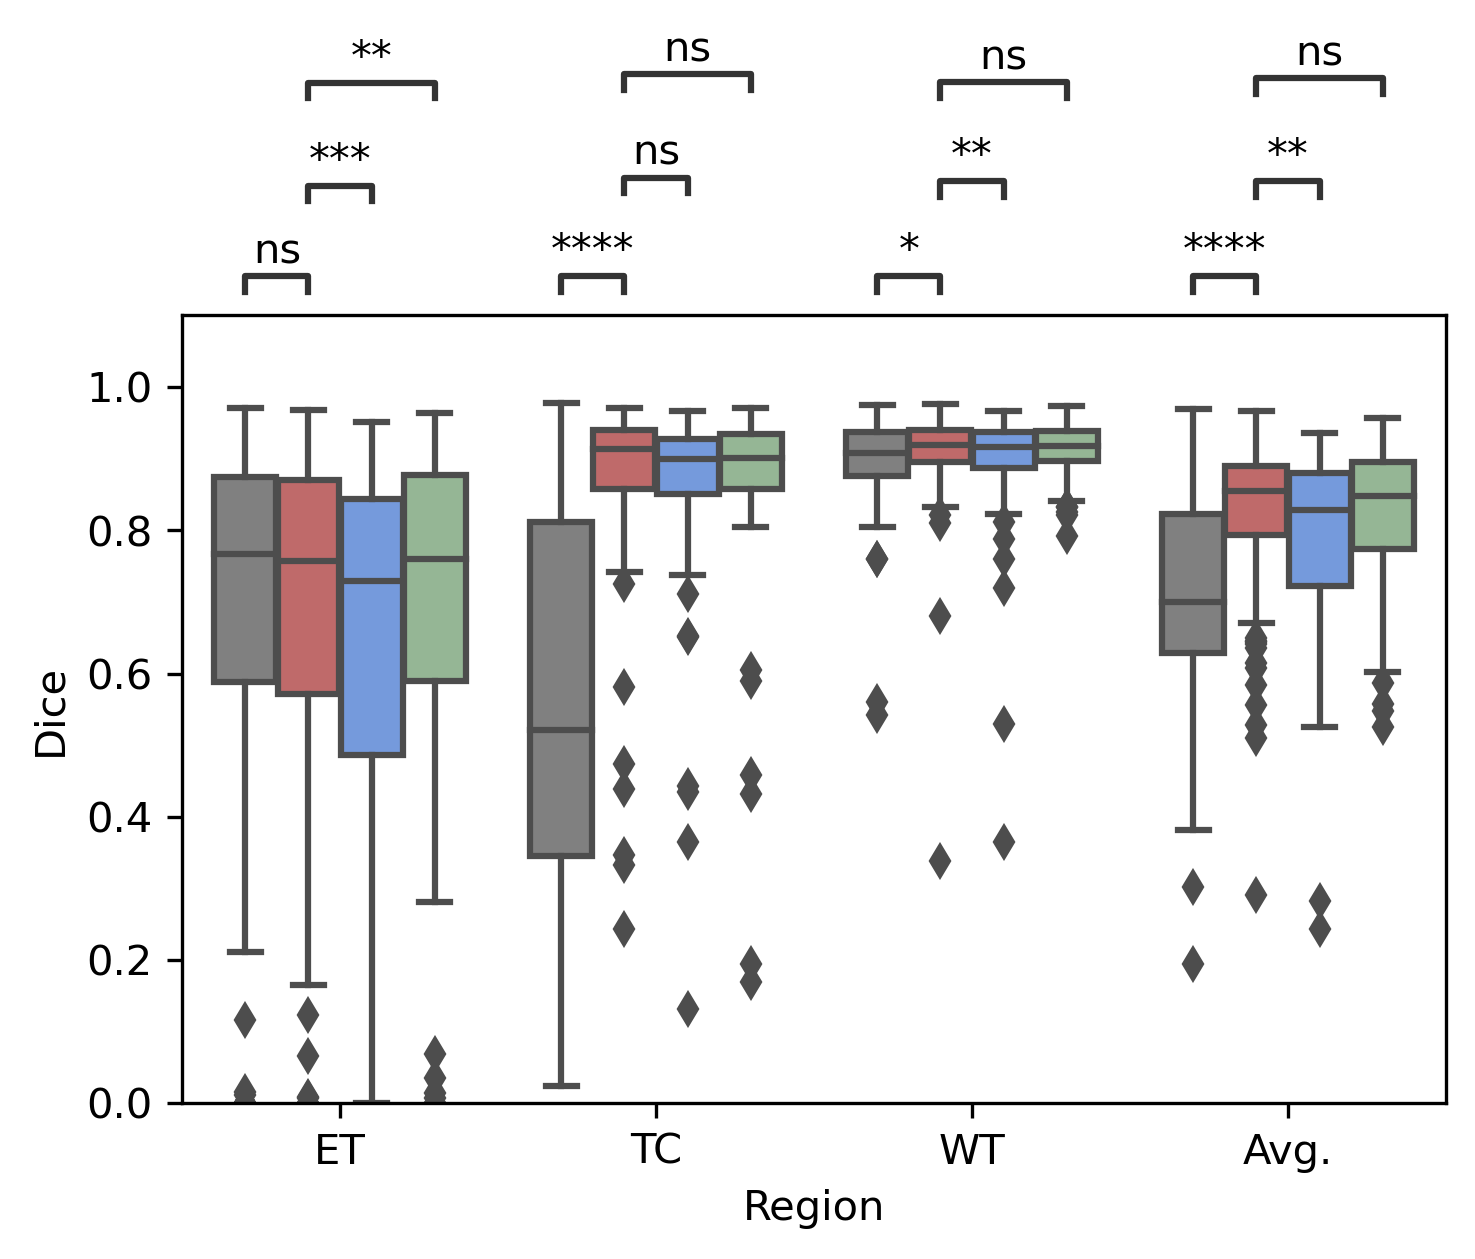
\includegraphics[width=0.48\textwidth]{Results_Unsupervised_Dice_noSmallET_fullset.png}
         %\caption{Tumor volume comparison}
         \label{fig:results_GRL}
     %\end{subfigure}
     \hfill
     %\begin{subfigure}[b]{0.48\textwidth}
         \centering
         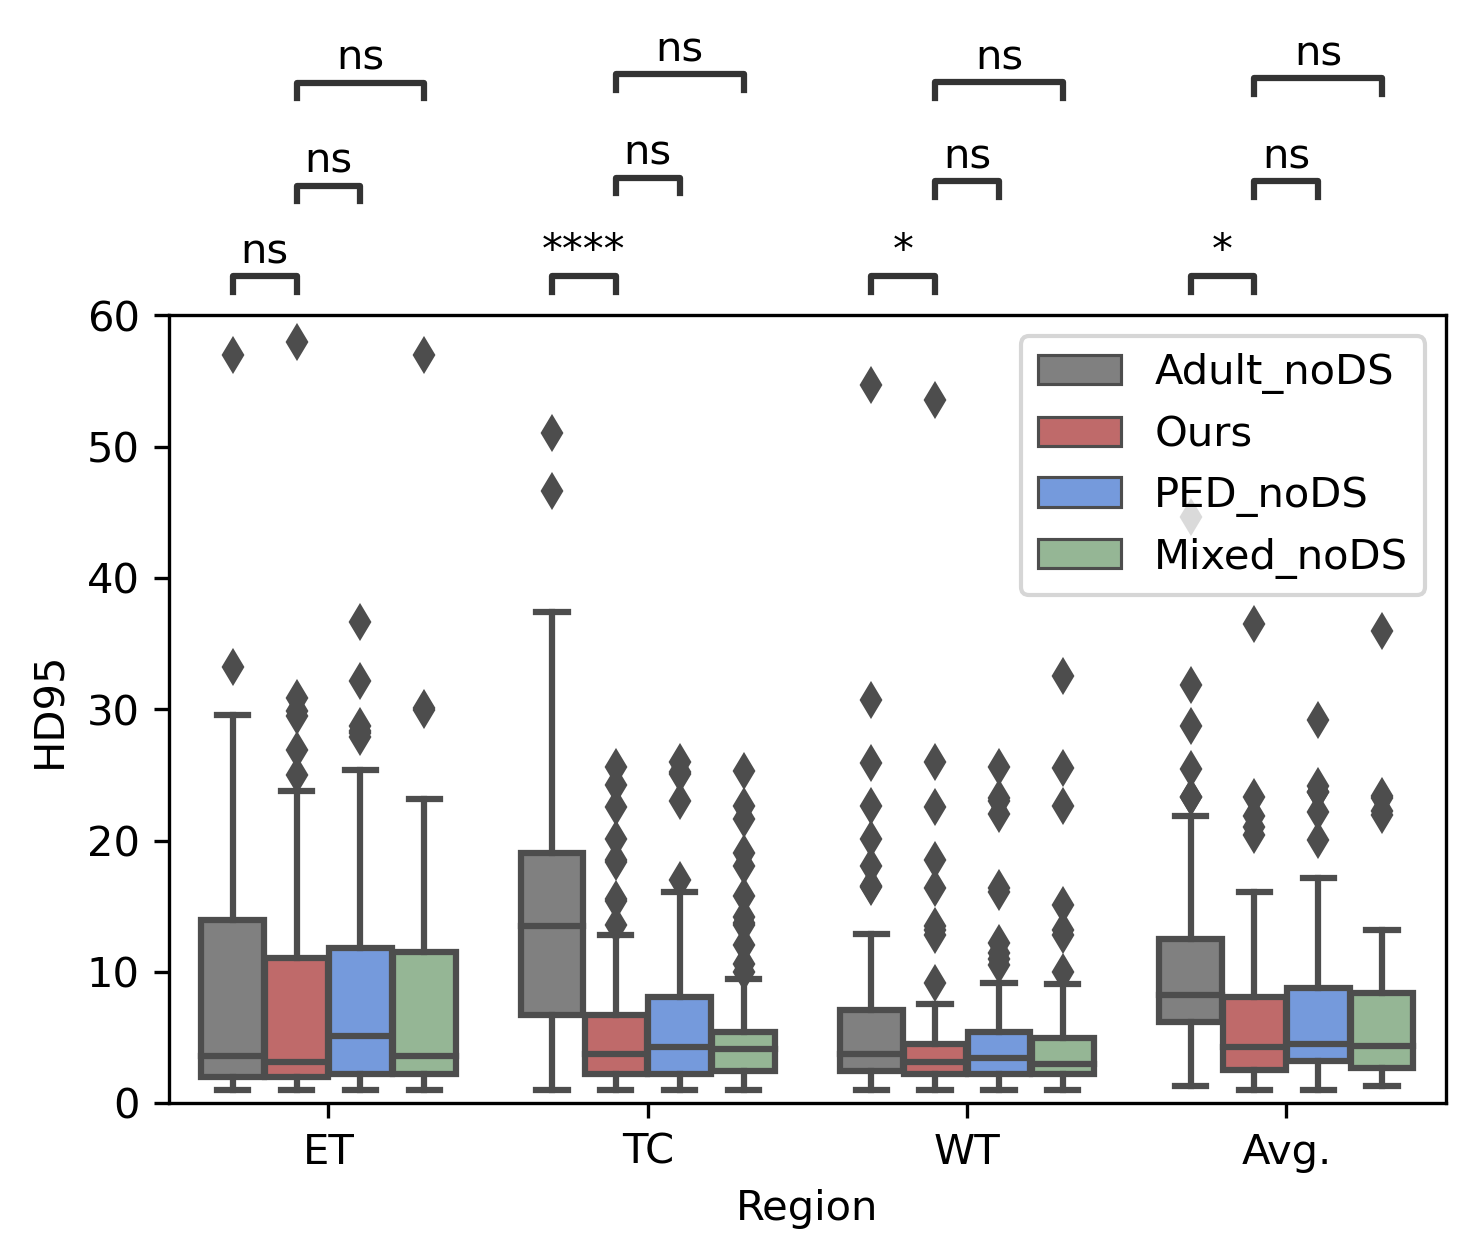
\includegraphics[width=0.48\textwidth]{Results_Unsupervised_HD95_noSmallET_fullset.png}
         %\caption{Tumor intensity comparsion}
         \label{fig:visual_illustration}
     %\end{subfigure}
\caption{Distributions of DSC (left) and HD95 (right) for Table \ref{tab:UDA_remove}. 
Pairwise t-tests were used to assess the statistical significance of differences between methods on $\mathcal{D}_{\text{PED}}^{\text{target}}$. 
} \label{fig:results}
\end{figure}

% \begin{figure}[t]
%      \centering
%      %\begin{subfigure}[b]{0.48\textwidth}
%          \centering
%          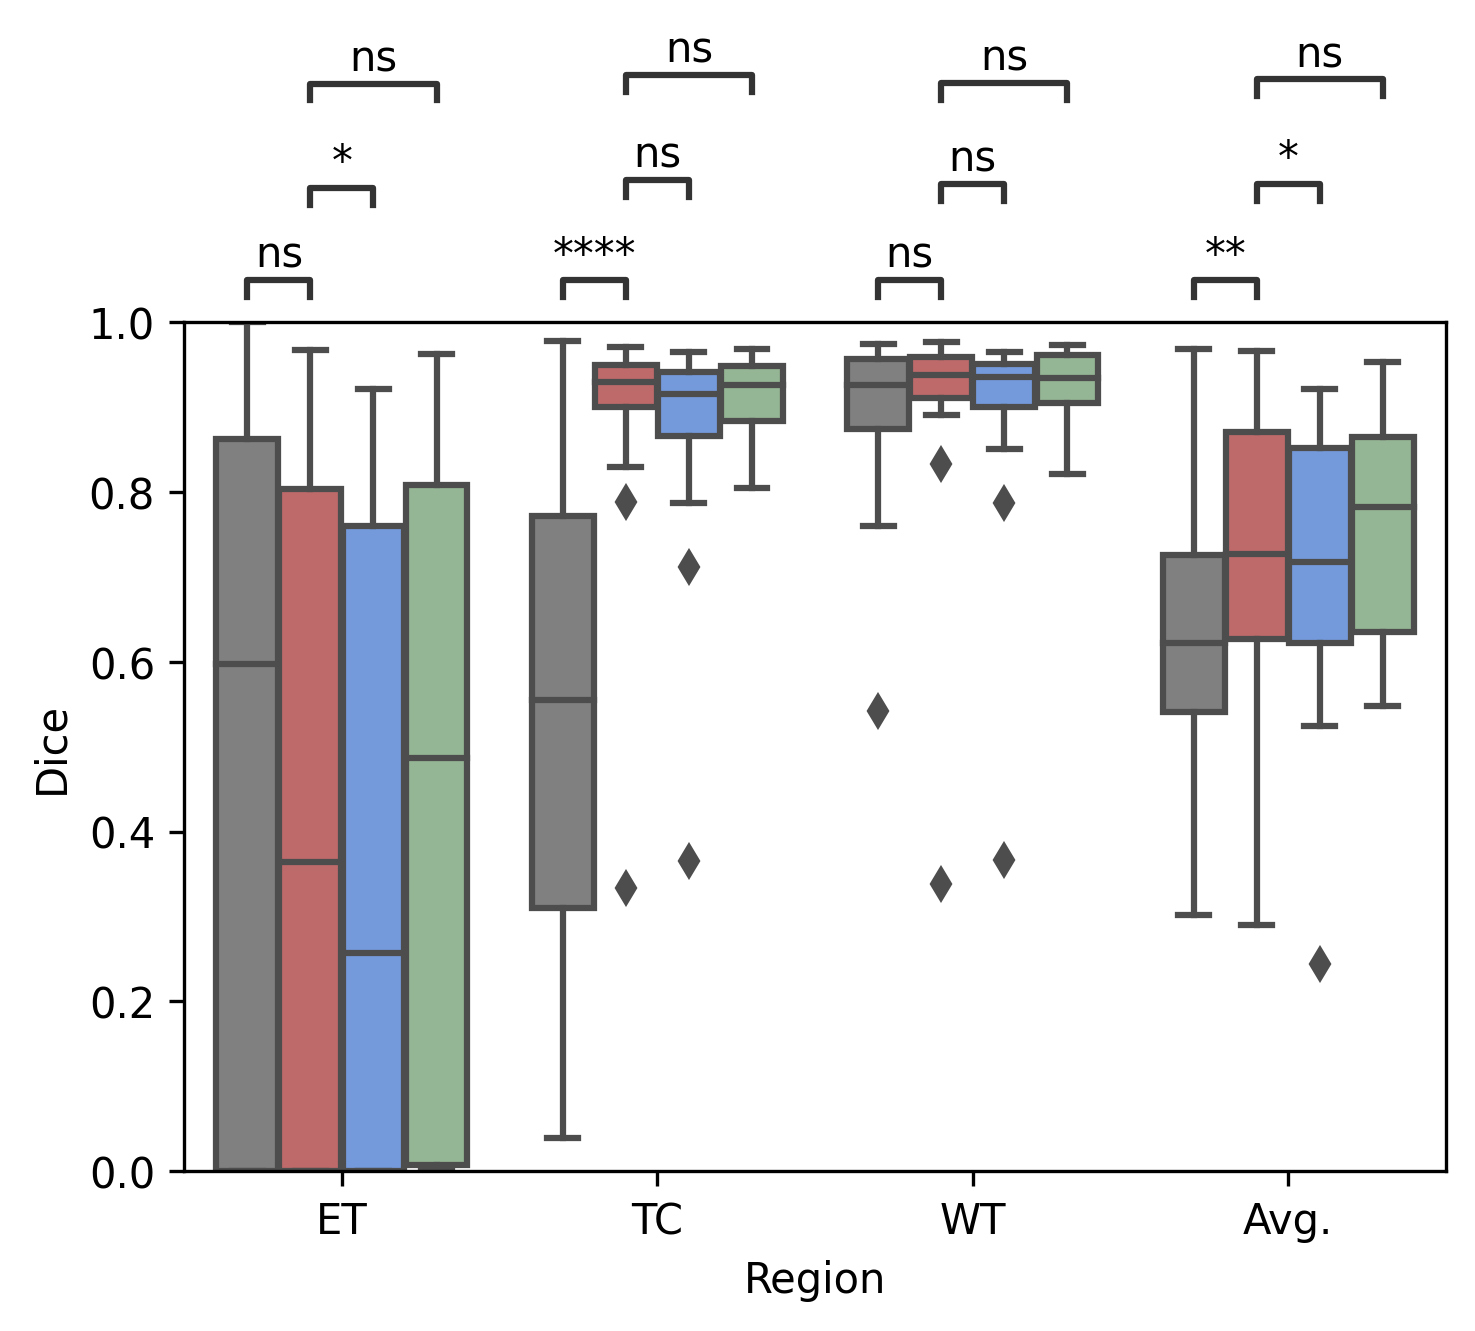
\includegraphics[width=0.48\textwidth]{Results_Unsupervised_Dice.png}
%          %\caption{Tumor volume comparison}
%          \label{fig:results_GRL}
%      %\end{subfigure}
%      \hfill
%      %\begin{subfigure}[b]{0.48\textwidth}
%          \centering
%          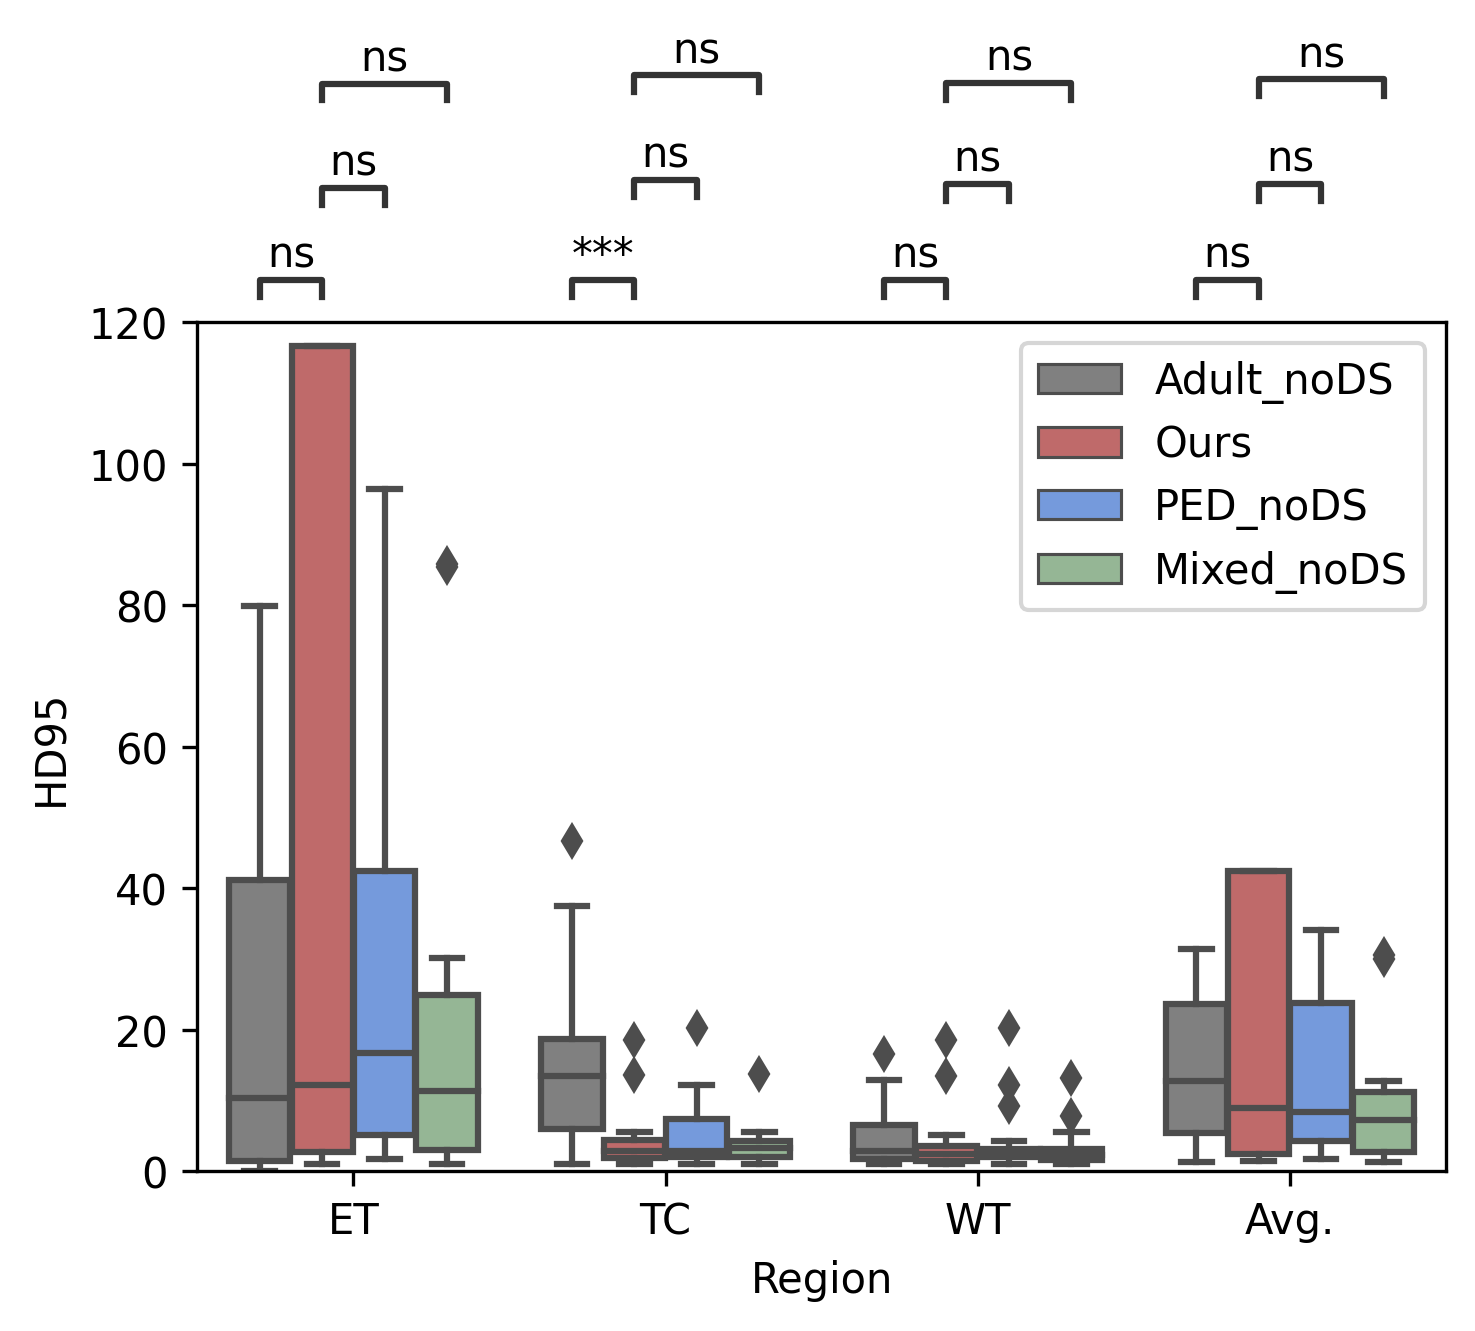
\includegraphics[width=0.48\textwidth]{Results_Unsupervised_HD95_legend.png}
%          %\caption{Tumor intensity comparsion}
%          \label{fig:visual_illustration}
%      %\end{subfigure}
% \caption{Distributions of Dice scores (left) and Hausdorff distance 95 (HD95) (right) for three baseline models and the proposed one. 
% Pairwise t-tests were used to assess the statistical significance of differences between methods on $\mathcal{D}_{\text{PED}}^{\text{test}}$. 
% } \label{fig:results}
% \end{figure}

% \begin{figure}[t]
%      \centering
%      %\begin{subfigure}[b]{0.48\textwidth}
%          \centering
%          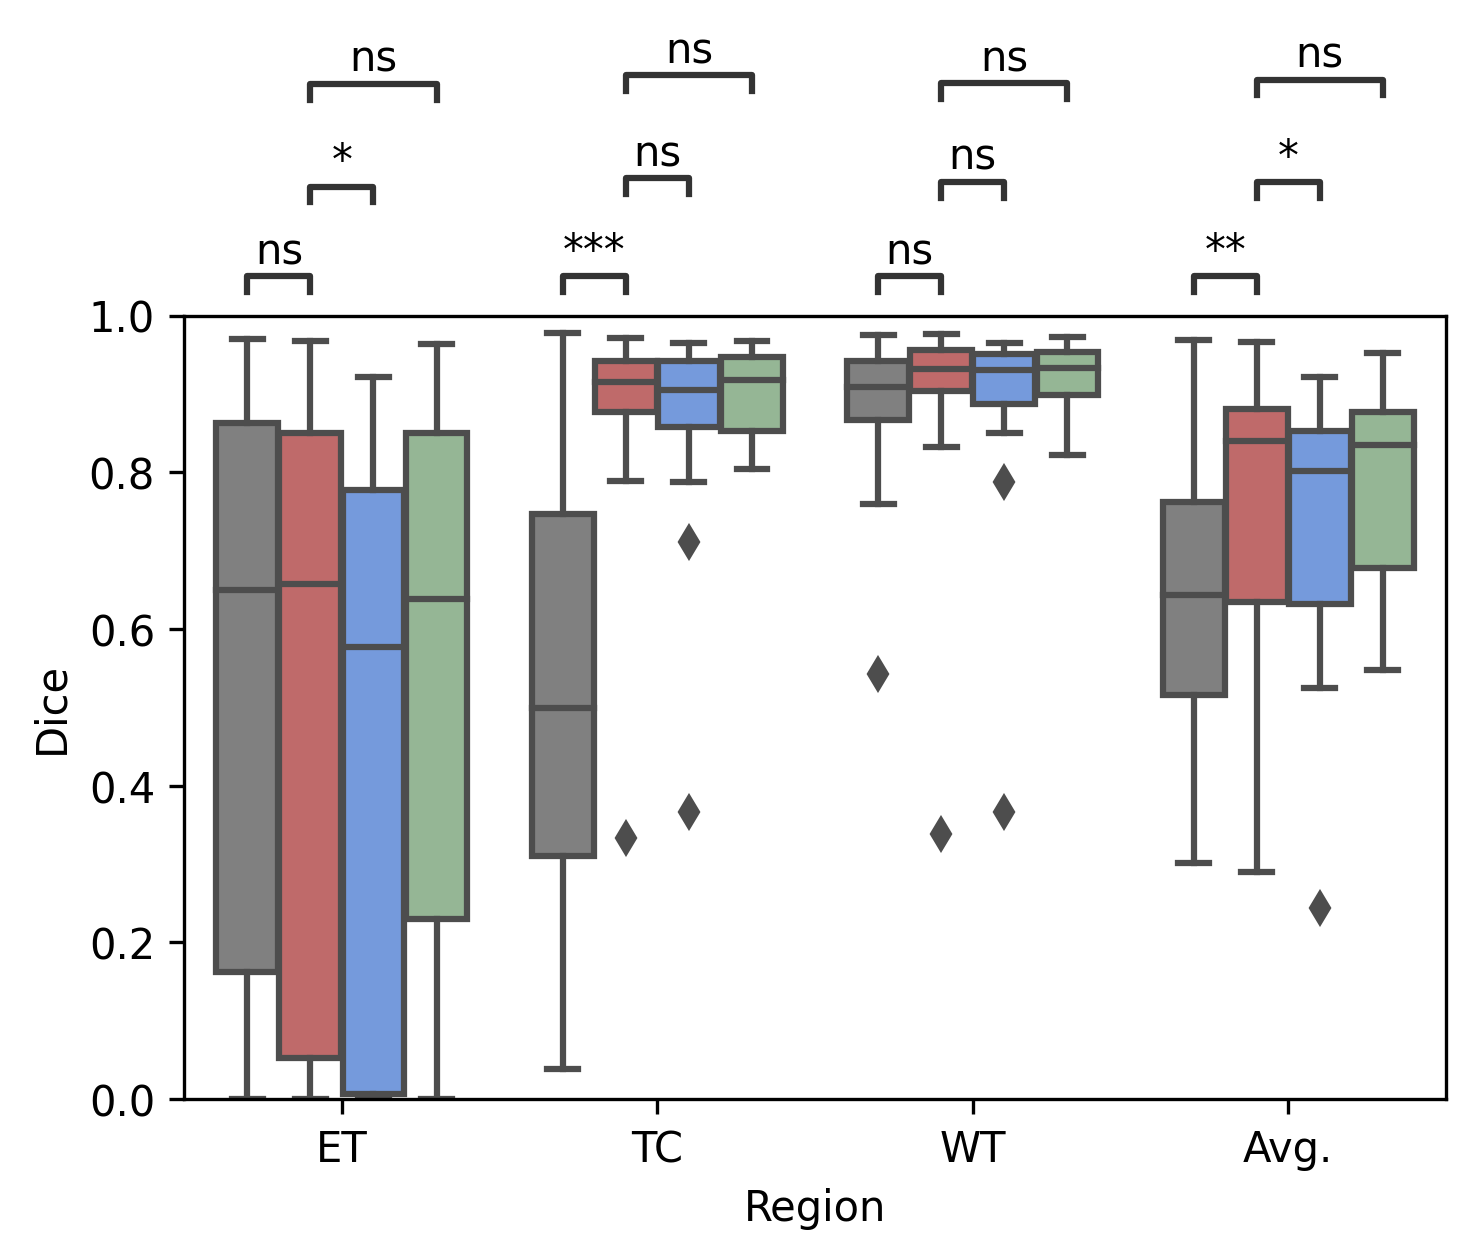
\includegraphics[width=0.48\textwidth]{Results_Unsupervised_Dice_removed4.png}
%          %\caption{Tumor volume comparison}
%          \label{fig:results_GRL}
%      %\end{subfigure}
%      \hfill
%      %\begin{subfigure}[b]{0.48\textwidth}
%          \centering
%          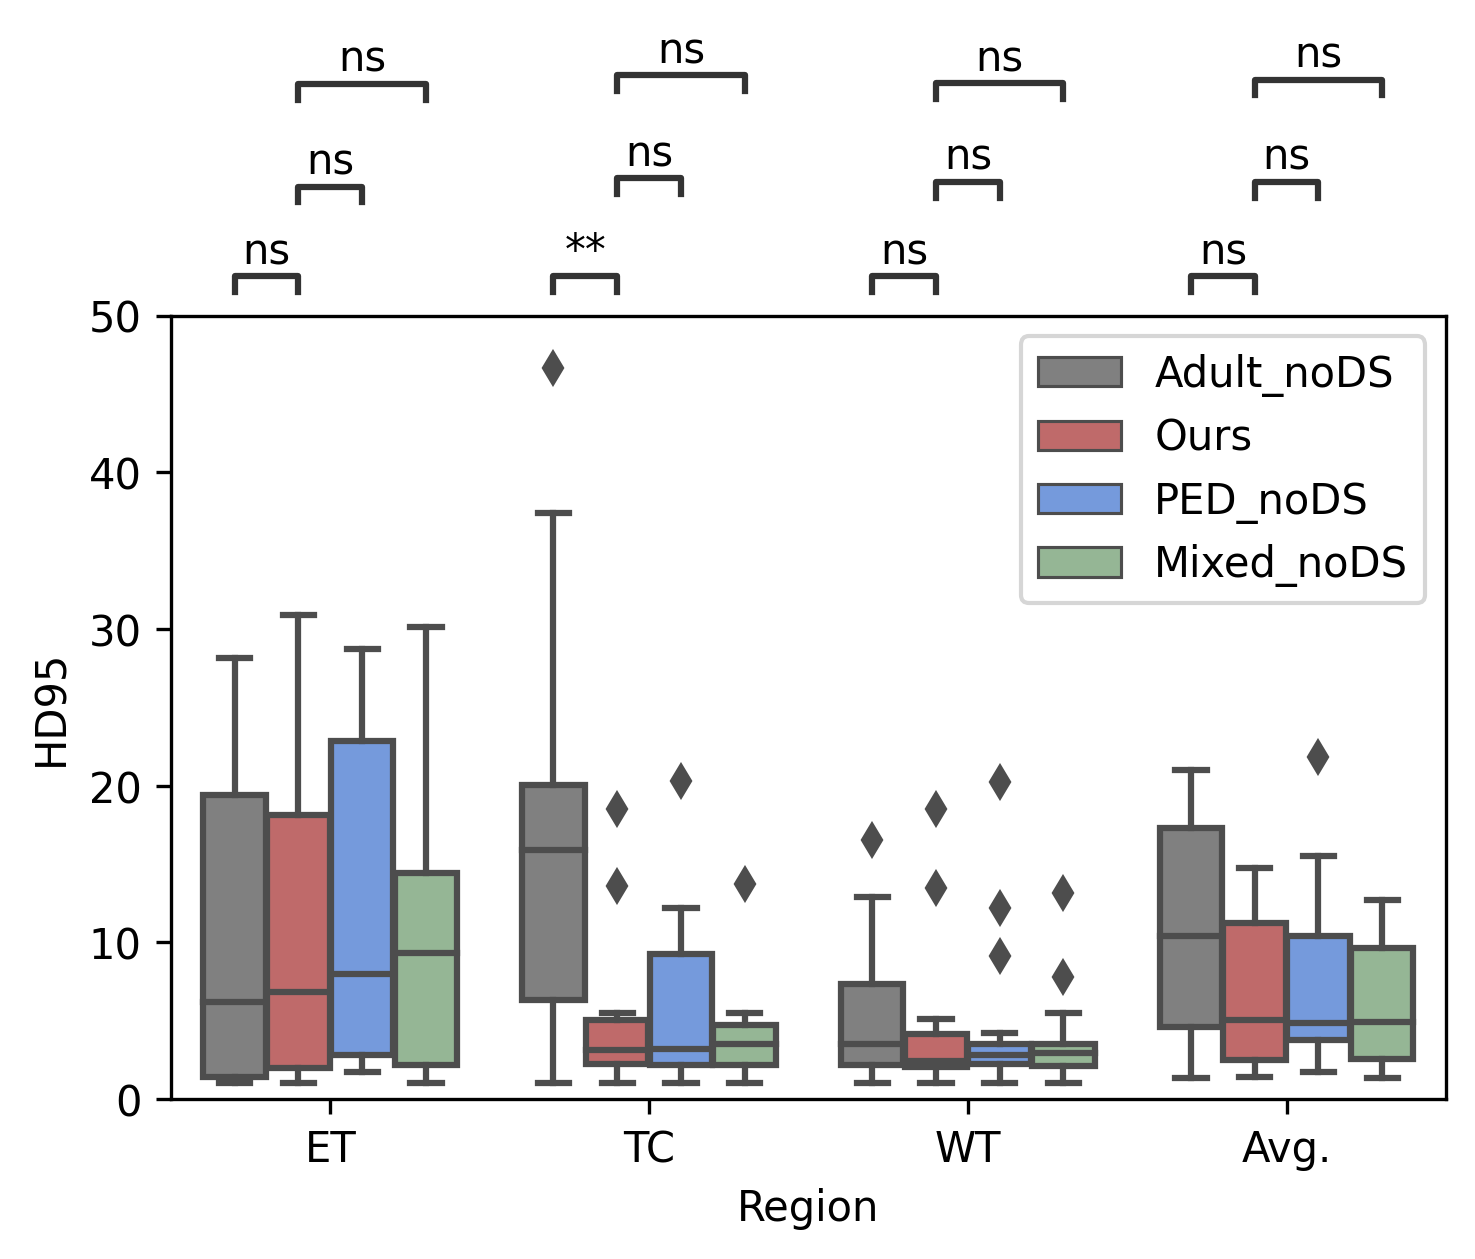
\includegraphics[width=0.48\textwidth]{Results_Unsupervised_HD95_removed4_legend.png}
%          %\caption{Tumor intensity comparsion}
%          \label{fig:visual_illustration}
%      %\end{subfigure}
% \caption{Distributions of Dice scores (left) and Hausdorff distance 95 (HD95) (right) for three baseline models and the proposed one. 
% Pairwise t-tests were used to assess the statistical significance of differences between methods on $\mathcal{D}_{\text{PED}}^{\text{test}}$. 
% } \label{fig:results}
% \end{figure}

% % median:
% \begin{table}[t]
% \caption{Comparison of methods on $\mathcal{D}_{\text{PED}}^{\text{test}}$ in medians.
% %Comparison of baseline and upper-bound models on $\mathcal{D}_{\text{PED}}^{\text{test}}$ described in Fig. \ref{fig:SDA}. 
% The models are ranked separately based on whether they have access to adult source data for training, or if deep supervision was deactivated (no DS). The best in each category is highlighted in bold.}\label{tab:SDA}
% \centering
% \begin{tabular}{ccccc|ccc}
% \hline
% \multirow{2}{*}{\textbf{Model}} & \multirow{2}{*}{\textbf{Trained on}} & \multicolumn{3}{c|}{\textbf{median DSC ($\uparrow$)}} & \multicolumn{3}{c}{\textbf{median HD95 ($\downarrow$)}} \\ \cline{3-8} 
%         & & ET & TC & WT & ET & TC & WT \\ \hline
% 1   & $\mathcal{D}_{\text{Adult}}^{\text{train}}$  & \textbf{0.615}&    0.650&    0.921&  \textbf{9.52}&    11.06&    2.91\\
% 2     & $\mathcal{D}_{\text{PED}}^{\text{train}}$ &  0.279&    0.926&    \textbf{0.939}&  17.34&    \textbf{3.00}&    2.83\\
% 3   & $\mathcal{D}_{\text{Adult}}^{\text{train}} \cup \mathcal{D}_{\text{PED}}^{\text{train}}$ & 0.460&    \textbf{0.940}&    0.917&    14.04&    \textbf{3.00}& \textbf{2.45}\\
% \hline
% 4      & $\mathcal{D}_{\text{PED}}^{\text{train}}$ &  0.333& \textbf{0.931}&     \textbf{0.941}&    11.00&    \textbf{2.91}&    2.83\\
% 5      & $\mathcal{D}_{\text{PED}}^{\text{train}}$ &  0.441&    0.902&    0.925& 11.82&    3.16&    2.83\\
% 6   & $\mathcal{D}_{\text{PED}}^{\text{train}}$ &  0.478&    0.923&    0.930&  15.07&    3.00&   2.91\\
% 7 & $\mathcal{D}_{\text{PED}}^{\text{train}}$ &  0.497&    0.910&    0.925& 16.12&  3.00&    \textbf{2.64}\\
% 8 & $\mathcal{D}_{\text{PED}}^{\text{train}}$ & \textbf{0.648}&    0.913&    0.935& \textbf{10.41}&   3.08&    \textbf{2.64}\\ \hline
% 1 (no DS) & $\mathcal{D}_{\text{Adult}}^{\text{train}}$  & \textbf{0.598}&    0.555&    0.926&  \textbf{10.28}&    13.43&    2.88\\
% 2 (no DS)   & $\mathcal{D}_{\text{PED}}^{\text{train}}$  & 0.257&    0.915&    \underline{0.936}&  16.68&   \textbf{2.91}&    2.83\\
% 3 (no DS) & $\mathcal{D}_{\text{Adult}}^{\text{train}} \cup \mathcal{D}_{\text{PED}}^{\text{train}}$  &  \underline{0.486}&   \underline{0.927}&    0.934&    \underline{11.38}&    \underline{3.24}&    \textbf{2.34}\\  \hline
% \textbf{UDA (ours)}  & $\mathcal{D}_{\text{Adult}}^{\text{train}} \cup \mathcal{D}_{\text{PED}}^{\text{train}}$  &    0.364&    \textbf{0.930}&    \textbf{0.938}&  12.12&    \textbf{2.91}&    \underline{2.45}\\ \hline
% \end{tabular}
% \end{table}

\begin{comment}
Table \ref{tab:UDA} shows the outcome of UDA, showcasing our proposed GRL-based approach. Specifically, we conducted a comparative analysis against three distinct baseline methods, each representing a different expected level of segmentation performance:
\begin{itemize}
    \item $\mathcal{D}_{\text{Adult}}^{\text{train}}$: This baseline represents the expected lower boundary of segmentation performance.
    \item $\mathcal{D}_{\text{Adult}}^{\text{train}} \cup \mathcal{D}_{\text{PED}}^{\text{train}}$: This baseline reflects the expected upper boundary of segmentation performance.
    \item $\mathcal{D}_{\text{PED}}^{\text{train}}$: This baseline serves as a reference for the segmentation performance achieved solely through training on pediatric cases.
\end{itemize}
\end{comment}


From the results of Table \ref{tab:SDA}, it is also evident that all tested methods have problems with segmenting ET: relatively low mean DSC and high mean HD95. Notably, there are significant disparities between median and mean metrics, with median values often considerably better than mean values (e.g., 4.12 median vs. 58.77 mean HD95 for model 1). %This may be attributed to the BraTS evaluation's tendency to penalize false positive predictions harshly, resulting in DSC=0 and HD95=374 when the reference segmentation is empty. However, 
As already mentioned, ET regions are usually very small or non-existent in pediatric cases. %, as shown in Fig. \ref{fig:domaindiff}. 
%Even, in some cases, that region is not existing; for instance, it's missing in 11 out of 99 cases in the BraTS-PEDs training set and in only 33 out of 1251 cases in the BraTS adult set. 
To assess the impact of small ET, we reevaluated models 1$^*$-3$^*$ and our UDA method without considering subjects with ET < 60 voxels (22 subjects were discarded, results shown in Table \ref{tab:UDA_remove}). %(results in 16 samples left). 
We observe that DSC and especially HD95 are largely improved for all methods in the ET region. This suggests that the considerable variation in ET segmentation performance is largely influenced by small region size. %Fig. \ref{fig:results} shows the distribution of DSC and HD95 and statistically significant differences among the four models from Table \ref{tab:UDA}. 
Moreover, the proposed UDA method is not statistically different from the practical upper bound model 3$^*$ (see Fig. \ref{fig:results}), except for the most challenging ET region in DSC metric. %It is clear that ET in pediatric tumors is the most challenging region for both supervised and unsupervised methods.

%The most interesting findings emerge from the comparative analysis between our proposed method utilizing the GRL and model 1, which is expected to be the lower bound of performance %the $\mathcal{D}_{\text{Adult}}^{\text{train}}$ baseline (i.e., representing the expected lower bound). 
%As illustrated in Figure \ref{fig:results_GRL}, the GRL model exhibits a significantly superior performance over the adult model across both Dice score and Hausdorff distance metrics for the tumor core region. Furthermore, in terms of DSC within the ET region, the GRL model surpasses the pediatric model, indicating the advantageous utility of our proposed GRL approach in refining segmentation predictions. This implication is further confirmed when analyzing the average segmentation performance across the three regions, indicating a significant improvement over the expected lower bound, while showing no significant difference with respect to the expected upper bound.


%%% Points to Discuss
%%% 1.a GRL vs Ped [ET] and GRL vs Adult [TC], GRL vs Mixed [Upper Bound] NS Dice
%%% 1.b GRL vs Adult [TC] HD95
%%% 2. Size and [Intensity] Shift across domains
%%%


\section{Conclusion}
%In a broader context, the statistical analyses conducted on the segmentation metrics suggest the efficacy of employing the GRL approach to enhance segmentation outcomes compared to a deep learning model solely trained on adult glioma volumes. Notably, the absence of a significant disparity between the performance of the GRL model and the mixed segmentation suggests the potential of GRL to achieve a performance level similar to that of the expected upper boundary model.

%These results underscore the promise of our GRL-based approach in not only surpassing the anticipated segmentation performance bounds but also in potentially achieving comparable performance levels to models trained on mixed datasets, thus corroborating its utility in improving brain tumor segmentation accuracy.

Our experimental results show that the proposed unsupervised domain adaptation approach performs similarly to supervised approaches for pediatric tumor segmentation. The main advantage of our approach is that it has the potential to be used in cases where expensive manual annotations are not available without a significant drop in performance.

% % Please add the following required packages to your document preamble:
% \begin{table}[]
% \begin{tabular}{cccc|ccc|ccc|ccc}
% \hline
% \textbf{Model}     & \multicolumn{3}{c|}{\textbf{mean LW DICE}}        & \multicolumn{3}{c|}{\textbf{mean LW HD95}}         & \multicolumn{3}{c|}{\textbf{median LW DICE}}      & \multicolumn{3}{c}{\textbf{median LW HD95}} \\ \cline{2-13} 
%                    & ET             & TC             & WT             & ET              & TC             & WT             & ET             & TC             & WT             & ET             & TC            & WT         \\ \hline
% Adult\_noDS        & \textbf{0.548} & 0.515          & 0.782          & \underline{115.08}    & 30.22          & 53.29          & \underline{0.679}    & 0.522          & 0.900          & \textbf{4.47}  & 13.49         & 3.74       \\
% PED\_noDS          & 0.396          & \textbf{0.846} & \textbf{0.876} & 170.65          & \textbf{13.03} & \textbf{12.10} & 0.380          & \underline{0.908}    & 0.918          & 189.45         & \underline{4}       & 3.32       \\
% Mixed\_noDS        & 0.468          & 0.812          & \underline{0.851}    & 143.72          & \underline{26.53}    & \underline{29.29}    & 0.462          & 0.901          & \textbf{0.920} & 20.47          & 4.12          & \textbf{3} \\ \hline
% DA\_nnUNet         & \underline{0.543}    & \underline{0.813}    & 0.838          & \textbf{103.53} & 31.24          & 30.76          & \textbf{0.687} & \textbf{0.914} & \underline{0.919}    & \underline{4.90}     & \textbf{3.61} & \underline{3.16} \\
% DA\_nnUNet\_PP\_et & 0.596          & -              & -              & 114.29          & -              & -              & 0.717          & -              & -              & 3              & -             & -          \\ \hline
% \end{tabular}
% \end{table}

% \begin{theorem}
% This is a sample theorem. The run-in heading is set in bold, while
% the following text appears in italics. Definitions, lemmas,
% propositions, and corollaries are styled the same way.
% \end{theorem}
% %
% % the environments 'definition', 'lemma', 'proposition', 'corollary',
% % 'remark', and 'example' are defined in the LLNCS documentclass as well.
% %
% \begin{proof}
% Proofs, examples, and remarks have the initial word in italics,
% while the following text appears in normal font.
% \end{proof}
 
\begin{credits}
\subsubsection{\ackname} This study was partially funded by Barncancerfonden (grant number MT2022-0008). We also thank Berzelius for their computational infrastructure. % the Swedish Childhood Cancer Foundation (grant number MT2022-0008). 
% and **** (grant number ****). We also thank *** for the use of their computational infrastructure in this project.

\subsubsection{\discintname}
The authors have no competing interests to declare.
% It is now necessary to declare any competing interests or to specifically
% state that the authors have no competing interests. Please place the
% statement with a bold run-in heading in small font size beneath the
% (optional) acknowledgments\footnote{If EquinOCS, our proceedings submission
% system, is used, then the disclaimer can be provided directly in the system.},
% for example: The authors have no competing interests to declare that are
% relevant to the content of this article. Or: Author A has received research
% grants from Company W. Author B has received a speaker honorarium from
% Company X and owns stock in Company Y. Author C is a member of committee Z.
\end{credits}
%
% ---- Bibliography ----
%
% BibTeX users should specify bibliography style 'splncs04'.
% References will then be sorted and formatted in the correct style.
%
\bibliographystyle{splncs04}
\bibliography{mybibliography}
%
% \begin{thebibliography}{8}
% \bibitem{ref_article1}
% Author, F.: Article title. Journal \textbf{2}(5), 99--110 (2016)

% \bibitem{ref_lncs1}
% Author, F., Author, S.: Title of a proceedings paper. In: Editor,
% F., Editor, S. (eds.) CONFERENCE 2016, LNCS, vol. 9999, pp. 1--13.
% Springer, Heidelberg (2016). \doi{10.10007/1234567890}

% \bibitem{ref_book1}
% Author, F., Author, S., Author, T.: Book title. 2nd edn. Publisher,
% Location (1999)

% \bibitem{ref_proc1}
% Author, A.-B.: Contribution title. In: 9th International Proceedings
% on Proceedings, pp. 1--2. Publisher, Location (2010)

% \bibitem{ref_url1}
% LNCS Homepage, \url{http://www.springer.com/lncs}, last accessed 2023/10/25
% \end{thebibliography}
\end{document}
